\documentclass[12pt, a4paper, oneside]{memoir}
\usepackage[english]{babel}
\usepackage[T1]{fontenc}
\usepackage[utf8]{inputenc}

\usepackage{amsfonts, amssymb, amsthm, bm, mathtools, multirow, siunitx, tikz}
% \usepackage[backref]{hyperref}

\usetikzlibrary{positioning, patterns}

\DeclareMathOperator*{\argmin}{argmin}
\DeclarePairedDelimiter{\ceil}{\lceil}{\rceil}
\DeclarePairedDelimiter\abs{\lvert}{\rvert}
\newcommand{\random}{\overset{\mathsf{r}}{\gets}}

\newtheorem{theorem}{Theorem}[section]
\newtheorem{proposition}[theorem]{Proposition}
\theoremstyle{definition}
\newtheorem{definition}[theorem]{Definition}
\newtheorem*{remark}{Remark}

\setcounter{tocdepth}{2}
\setcounter{secnumdepth}{2}

\chapterstyle{article}

\begin{document}

\tableofcontents*

\chapter{Introduction}\label{ch:intro}

Cryptography is the discipline in which techniques for achieving secure communications are studied. Historically, information was hidden from adversaries by scrambling its contents with an algorithm that received a single key as input. The possession of the key is paramount in obtaining the original information, such that a well-designed algorithm would prevent its discovery by any means other than the usage of the specific key. This practice persists nowadays with increasingly complex algorithms, and is known as symmetric cryptography, since said key can \emph{encrypt} plain text or \emph{decrypt} the corresponding ciphered text.

Evidently, storage, transportation and communication of such keys are sensitive procedures. More precisely, an insecure channel can yield a cryptographic key due to a logistical failure or a malicious actor that controls part of the channel. With the advent of computers and the consequent facilitation of communications, this situation became apparent to a greater extent. In order to solve this problem, a new paradigm of cryptography was introduced in~\cite{Diffie:197611}, called asymmetric, or \emph{public-key cryptography}. Within this system, an entity holds a key pair, composed of a private key and a public key. 

Key pairs are mathematically bound to a computationally hard to solve problem, which is the basis for the security of the resulting cryptosystem. In other words, it should be computationally hard to recover a private key from its corresponding public key. There exist various methods of constructing a public-key cryptosystem, with direct consequences on its resulting security, performance and assurance of distinct properties. Particularly, public-key cryptography provides a digital alternative to handwritten signatures, which are one of the ubiquitous ways to ensure trust when a contract is sealed between parties. 

Signatures in the form of seals, stamps, or ink drawings present various logistical and security shortcomings. For instance, individuals are advised to be physically present to sign any documents, for they cannot be truthfully identified otherwise. Additionally, this kind of personal calligraphy or symbolism can be forged with little effort. A modern solution is found within mathematical frameworks known as \emph{signature schemes}, that enable explicit assertions on the security of signatures. 

A vibrant discipline of public-key cryptography, signature schemes are often associated with digital systems, in which transit of sensitive messages is again expected to be secure. The initial public discovery of digital signature schemes is given in~\cite{Rivest:197802} and still widely used at the time of the writing. The RSA signature scheme is based on the difficulty of integer factorization. Other popular schemes, such as Ed25519~\cite{Bernstein:201208}, are based on the difficulty of calculating a discrete logarithm. There is no known polynomial time algorithm to solve such problems on a conventional computer.

Classical computers are electronic in nature, using circuits to perform computations. However, a new paradigm has emerged in the form of quantum computers, in which computations are performed outside the scope of classical mechanics. Although these computers are physically hard to implement, algorithms that make use of quantum phenomena have already been proposed and present a provable speed-up compared to classical computers. One of these algorithms~\cite{Shor:199710} simplifies the complexity
of factoring integers and calculating discrete logarithms. Consequently, it can be theoretically used to break widely used signature schemes.

\emph{Post-quantum cryptography} addresses this issue by defining public-key cryptosystems which are either not known to be affected by quantum computers, or provably so~\cite{Bernstein:2008}. Such algorithms operate on classical computers, and as such, post-quantum cryptography does not encompass quantum algorithms for cryptography. While a recent discipline, post-quantum cryptography has generated considerable research effort with the intent of replacing current cryptosystems with comparatively practical, quantum-safe counterparts. A noteworthy example is the standardization call by the National Institute of Standards and Technology (NIST)~\cite{Alagic:201901,Alagic:202007}, which houses proposals based on several distinct mathematical structures as the theoretical bases for underlying problems.

\subsubsection{Scope of our research.}

It is known that the difficulty of solving polynomial systems over multiple variables does not change in the quantum setting, as discussed in Section~\ref{sec:mult}. The discipline of cryptographic primitives based on this problem is known as \textit{multivariate public-key cryptography}, or simply multivariate cryptography. Families of multivariate cryptosystems are defined according to the usage of finite fields in the computations. This enables the focus on specific improvements, such as trade-offs between key and signature sizes, or larger security parameters.

Multivariate cryptosystems are extremely time- and space-efficient when operating over messages. However, public and private keys are defined by large polynomial systems with little opportunity for compression or sparseness. Large key sizes frequently impose constraints on the use of signature schemes in devices of limited storage and processing power. In multivariate cryptography, keys are often orders of magnitude larger than the ones used in conventional signature schemes.

In this thesis, we solely discuss multivariate signature schemes based on the Oil--Vinegar principle. More precisely, UOV~\cite{Kipnis:199904} and its generalization Rainbow~\cite{Ding:200506} receive primary attention. Such schemes perform computations over a single field and present a balanced nature and simple, elegant definitions. Consequently, signature schemes of a different structure such as HFE~\cite{Patarin:199605}, or multivariate public-key encryption schemes such as SRP~\cite{Duong:201607}, are not addressed. Furthermore, we specifically discuss strategies for reducing key sizes of Rainbow-like signature schemes and the security implications of such methods.

\subsubsection{Contributions and outline of this thesis.}

We intend to provide the reader with a complete overview of the mathematical background necessary to understand the family of Oil--Vinegar signature schemes and related discussions of its security. Thus, in Chapter~\ref{ch:math}, we start by introducing the mathematical concepts used in the description of such schemes, and then proceed to present the UOV and Rainbow signature schemes. 

We develop upon Rainbow on Chapter~\ref{ch:eta}, where we propose a novel approach to reduce the private key size with three possible implementations. We discuss the consequences of our modifications through a statistical analysis and show its consequences on key pair sizes for several parameter sets. The contents of this chapter were published as paper in a peer-reviewed conference proceedings~\cite{Zambonin:201907}. 

In Chapter~\ref{ch:attack}, we show that our modification is susceptible to a key recovery attack, and discuss mitigations in order to preserve some reduction in key sizes while maintaining reasonable levels of security. Finally, in Chapter~\ref{ch:conc}, we summarize and finish our discussion with pointers to open research topics.

\section{Related work}\label{sec:related}

In this section, we make use of the previously well-defined boundaries with regards to the scope of our work in order to perform the necessary search in the literature. We recall that our main object of study are digital signature schemes which make use of Oil--Vinegar polynomials in their construction. More precisely, it is known that key sizes for instances of such schemes are currently impractical. Thus, we inspect works that aim to mitigate this situation, in order to identify common strategies and pitfalls.

We conduct our literature review by making use of the Google Scholar meta-indexer tool, which covers most scientific literature providers, and allows the user to efficiently delimit the desired scope. We identify three critical works in the history of signatures based on Oil--Vinegar polynomials~\cite{Patarin:199709,Kipnis:199904,Ding:200506} and conduct the search over works that directly cited at least one of those. We consider only publications written in English that additionally are not patents. From this set, we select relevant papers and present a summary below.

\subsection{Improvements to private key size}\label{subsec:priv}

Rainbow is evidently the most popular multivariate signature scheme based on Oil--Vinegar polynomials. However, schemes of that class that feature modifications with the intent of reducing key sizes have been proposed even before Rainbow itself was proposed. Chronologically, the first schemes with this feature are tame transformation schemes (TTS)~\cite{Chen:200210}, in which equations of the private key are required to present a minimum level of sparseness. This strategy was attacked with various algebraic techniques, e.g. MinRank and the UOV attack, and corrected several times, as summarized in~\cite{Ding:200604}.

A similar idea introduced at roughly the same time are stepwise triangular systems (STS) in their generalized form~\cite{Wolf:200603}. The inherent shape of their private keys, hence the name, is derived from the fact that there are restrictions in the choice of variables for each polynomial in the central map, on top of the Oil--Vinegar construction. This strategy indirectly enables a reduction in private key size. STS were found to be insecure in the same work that designed the general classification. The authors propose an inversion attack that recovers the original message from its corresponding signature, and additionally show that it is possible to build an equivalent private key.

STS and TTS were later found to be specialized cases of the general Rainbow construction~\cite{Ding:200806}, due to their similarities in the usage of layers and the central map inversion procedure. These advances, as well as further cryptanalysis of Rainbow itself~\cite{Billet:200609} with the MinRank attack, led to the proposal of new parameters for TTS and Rainbow~\cite{Ding:200806}. This was achieved through the creation of the Rainbow band separation attack, an extension of the UOV reconciliation attack. Further modifications were suggested to salvage the previous schemes~\cite{Tsujii:201005}, but every such variant was broken through a key recovery attack~\cite{Thomae:201207} which stems from the generalization of the theory of equivalent keys.

Equivalent keys are explained in more detail in Section~\ref{sec:mult}, in which it is shown that the bipolar construction leads to a large amount of redundancy in the key space. Indeed, this fact is usually applied to find inconsistencies in the security of proposed schemes, as seen in this section. However, a consequence of this theory is that the associated matrices of the affine transformations that hide the central map structure may be thoroughly simplified. This is explored in~\cite{Czypek:201209}, for instance, to insert instances of UOV and Rainbow into low-resource devices.

We note that in the case of STS and TTS, reducing the private key was not the main intention of the authors, and it is thus not trivial to estimate such gains through direct comparison to Rainbow. Indeed, the reduction of keys is a known strategy to increase the performance of operations on signatures. On the other hand, there are several proposals in the literature which focus on the modification of Rainbow with the sole purpose of reducing key sizes. This motivation partially stems from recent efforts to present quantum-safe cryptography as a valid alternative to traditional digital signature schemes~\cite{Bernstein:2008}.

A variant of Rainbow based on quadratic forms~\cite{Yasuda:201306} features a trade-off between private key and public key size in order to increase the performance of the signature generation step. It replaces the central map with a small invertible matrix, reducing the size of the private key by up to $91.2\%$ and increasing the public key threefold. However, it was found to be insecure directly afterwards~\cite{Hashimoto:201410} by algebraic cryptanalysis leading up to the discovery of equivalent keys.

NC-Rainbow~\cite{Yasuda:201202} is proposed as a novel strategy, based in non-commutative rings, used to reduce a private key by up to $75\%$. However, it was shown by independent researchers to be insecure through a combination of rank attacks and the UOV attack~\cite{Thomae:201209,Hashimoto:201302}. The variants MB-Rainbow~\cite{Yasuda:201305} and NT-Rainbow~\cite{Yasuda:201404} are based on the insertion of, respectively, sparse diagonal and non-triangular matrices into the central map, to reduce the private key by up to $40\%$. The authors merged MB- and NC-Rainbow into a single scheme MNT-Rainbow~\cite{Yasuda:201409}, shortening private keys by up to $76\%$. 

The parameters of MB- and NT-Rainbow were deemed vulnerable to the Rainbow band separation attack by the authors of~\cite{Peng:201706}. In this work, Circulant Rainbow is also proposed, which gives a reduction of the private key by up to $45\%$, due to the concept of rotating relations introduced to the central map. This approach and its analogous UOV variant~\cite{Peng:201803} were broken shortly after with an application of the UOV attack by the authors of~\cite{Hashimoto:201903}. The strategy of MB-Rainbow was applied to UOV in~\cite{Tan:201511}, alongside with the replacement of certain parts of the private key by values generated through linear recurring sequences. While these strategies reduce the private key by up to $89.1\%$, they were found to be insecure~\cite{Park:201803} with the discovery of an attack to efficiently find equivalent keys. 

In the ELSA variant~\cite{Shim:201712}, a hidden layer of quadratic equations is inserted to simplify the private key and thus achieve a reduction of up to $88\%$ in its size. Nonetheless, it was found that such structure introduced shortcuts enabling an attacker to find equivalent keys~\cite{Hashimoto:201909}. The SOV signature scheme~\cite{Shim:202001} is built by preventing overlap of quadratic terms in the central map and assigning a specific rank to the matrices associated with its polynomials, reducing private key size by up to $91.9\%$.

Some non intrusive approaches are also found in the literature. The authors of Lite-Rainbow-0~\cite{Shim:201512} propose the replacement of the entire private key with a small pseudorandom number generator (PRNG) seed. This shortens the private key by a factor of approximately $99.8\%$, but evidently increases the cost for signature generation. In~\cite{Borges:201209}, it is suggested to use the RC4 stream cipher in the private key generation of UOV~\cite{Borges:201209}, presenting analogous decreases in the private key size but no noticeable effects on signature generation performance. Such approach also works with Rainbow~\cite{Dornelles:201910}. A similar result is also given in another work~\cite{Seo:201403}, in which AES-CTR is employed as the PRNG of choice.

The precomputation of UOV signatures such that the private key is not required is proposed in~\cite{Chen:201603}. This ``online-offline'' approach does not modify the key itself but can be used to yield signatures without the need to load the private key, thus reducing total storage requirements. Finally, the proposal by the authors of~\cite{Zambonin:201907} is discussed in more detail in~\cite{Bittencourt:201911} and further expanded in Chapter~\ref{ch:eta}.

\subsection{Improvements to public key size}\label{subsec:pub}

In the case of modifications to the public key, there are not as many approaches as for private keys. The first strategy is based on the method of field lifting, where the resulting LUOV scheme~\cite{Beullens:201712} has the central map and public key lifted to an extension field, such that coefficients of those polynomial systems are now smaller. This is a trade-off between public key size and signature size, but it is general enough to be compatible with other public key reduction strategies. LUOV has been submitted to the standardization process by NIST~\cite{Alagic:201901}, and it was subsequently attacked with a new strategy based on differentials between the base and extension fields~\cite{Ding:201912}. Due to this fact, it was not considered to the third round of the process~\cite[Section~3.24]{Alagic:202007}. An extension of the LUOV proposal to Rainbow~\cite{Duong:202003} was submitted before any attacks were known, but it is unclear if it is affected by the differential method.

A development by the name of BACUOV~\cite{Szepieniec:201908} forces matrices representing the central map and public key to be block-anti-circulant. This allows for a compression of both keys in the key pair, although only public key size improvements are featured on the aforementioned work. Still, the authors of~\cite{Furue:202004} show that the security levels of BACUOV are smaller than originally claimed through manipulation of the public key and the application of the UOV attack.

We also classify the work in~\cite{Szepieniec:201706} as relevant, since it is a general method motivated by the context of public key infrastructures, in which the size of a public key and signature bundle must be minimized. The strategy, which consists of a trade-off between signature and public key sizes with their combined length still reduced, was initially proposed for multivariate trapdoors, and subsequently generalized~\cite{Beullens:201808} to work in different security models and other signature schemes.

The approach proposed in~\cite{Petzoldt:201006} is, to the best of our knowledge, the most scrutinized method for public key reduction without compromises to the signature size. It was originally used to create cyclic UOV, which has cyclic relations built into the public key, reducing its size by up to $80.5\%$. It explores the fact that specific parts of the public key do not contribute to the security of the scheme, and thus can be structured at will. A detailed discussion of the mathematical relations that allow for this class of improvements, as well as its limitations, are shown in Section~\ref{sec:mod}. Schemes that make use of this framework are discussed below. 

A strategy analogous to a manipulation between base and extension fields is given in~\cite{Petzoldt:201109}. The resulting scheme is 0/1 UOV, in which coefficients of the public key are in $\mathbb{F}_{2}$. The proposal consists of creating the matrix associated with the structured part of the key according to a graph structure. Such graph describes a relationship of coefficients that, while sparse, does not facilitate known attacks over UOV, reducing the public key size by up to $88.6\%$. However, it is unknown if this proposal can be extended to Rainbow.

The CyclicRainbow variant~\cite{Petzoldt:201012} is a direct extension of cyclic UOV. It is featured on the Rainbow submission for the second round of the standardization process conducted by NIST~\cite{Ding:201901}. It reduces public keys by up to $53.8\%$, and the associated key generation algorithm is comparably efficient to Rainbow~\cite{Petzoldt:202004}. Another strategy is the usage of linear recurring sequences to generate such unimportant parts of the public key. It is summarized in two works~\cite{Petzoldt:201103,Petzoldt:201211} and reduces public keys by up to $56.6\%$.

\subsection{Improvements to total key pair size}\label{subsec:both}

Additionally, there are works in the literature which manage to reduce both private and public key sizes through novel strategies. The authors of LWRS~\cite{Zhang:201208} create a scheme with low-resource devices in mind. The left affine transformation of the usual bipolar construction is dropped, and the ``minus'' method~\cite[Subsection 3.2.1]{Wolf:200511} is applied to the public key, of which the last $\delta$ equations are removed. Precisely $m (m + 1)$ field elements are removed in the private key, and a reduction factor of $1 - \frac{\delta}{m}$ is achieved on the public key. 

A modification that consists of adding cross-terms of oil variables in the last layer to the last two layers of Rainbow is proposed in~\cite{Tan:201603}. With this method, which is also applicable to UOV, the authors are able to reduce Rainbow private and public keys by up to $46.2\%$ and $36.8\%$, respectively. The matrices associated with the public and private keys of the HUFU-UOV scheme~\cite{Tao:201905} have special Toeplitz and circulant constructions, which for instance enables the compression of the public key by up to a factor of $4.5$.

The variant known as Cubic UOV~\cite{Nie:201511} introduces a number of cubic polynomials in the central map of the private key. A consequence is that both keys of this variant are smaller when comparing to the original UOV scheme, although the focus of the original work is on reducing public keys. However, it was found to be insecure~\cite{Hashimoto:201712} through the recovery of equivalent keys. Repaired versions CSSv and SVSv were proposed~\cite{Duong:201611}. The former removes most cubic polynomials and further unnecessary structure from the key pair, while the latter does not feature cubic polynomials at all and uses a sparse central map. These proposals achieve further decrease in key sizes, being comparable to Rainbow in some instances. However, independent researchers found both strategies to be flawed~\cite{Shim:201711,Hashimoto:201712} to HighRank and key recovery attacks using equivalent keys.

It is evident that there have been commendable efforts in the creation, validation and correction of signature schemes based on Oil--Vinegar polynomials. However, it should be noted that most works which introduce any kind of structure into the key pair eventually succumb to algebraic cryptanalysis. It is thus our intention with this review to suggest that such approaches should be applied with caution, and to suggest a distinct approach, as presented in Chapter~\ref{ch:eta}.

\chapter{Mathematical background}\label{ch:math}

In this chapter, we give the mathematical toolbox necessary in order to fully comprehend the remainder of this work. In Section~\ref{sec:algebra}, we define basic algebraic structures that rule the operations of mathematical structures within our scope. In Section~\ref{sec:mult}, a brief panorama of concepts associated with multivariate cryptography is given. In Section~\ref{sec:ov}, we discuss the Unbalanced Oil and Vinegar signature scheme, its generalized form Rainbow, and how this trapdoor is impacted by cryptanalytic methods.

We use the following symbols throughout this work. The symbol $\random$ is read as ``chosen randomly from''. The symbol $\approx_{\varepsilon}$ means that two numbers are equal within a precision of $\varepsilon$. The usual function composition is given by the symbol $\circ$, and the inverse of a function $f$ is given by $f^{-1}$. The usual mean and standard deviation functions for a set of elements $S$ are respectively given by $\mu(S)$ and $\sigma(S)$. The concatenation of two elements up to context is given by $\mid\mid$.

\section{Algebraic structures}\label{sec:algebra}

We define below the elementary algebraic structures known as groups, rings, fields and vector spaces. We make this clear distinction since there are several underlying structures used in multivariate cryptography which, for instance, operate on the context of a finite field but actually form only a group or ring. Most definitions are taken from~\cite{Dummit:2003} and~\cite{Mullen:2013}, and we refer the reader to these references for proofs of the facts given below.

\begin{definition}
  Given a set $G$ and any $g_{1}, g_{2}, g_{3} \in G$, a \emph{binary operation $\star$ on a set $G$} is a function $\star : G \times G \to G$, where we denote $\star(g_{1}, g_{2})$ as $g_{1} \star g_{2}$. A binary operation $\star$ on a set $G$ may also satisfy the following conditions, for all $g_{1}, g_{2}, g_{3} \in G$:
  
  \begin{itemize}
    \item It is \emph{associative} if $g_{1} \star (g_{2} \star g_{3}) = (g_{1} \star g_{2}) \star g_{3}$.
    \item It is \emph{commutative} if $g_{1} \star g_{2} = g_{2} \star g_{1}$.
    \item It is \emph{closed under $G$} if $g_{1} \star g_{2} \in G$.
  \end{itemize}
\end{definition}

\begin{definition}
  Given a set $G$, any $g \in G$ and a binary operation $\star$ on $G$, a \emph{group} is an ordered pair $(G, \star)$ that satisfies the following axioms:
  
  \begin{enumerate}
    \item The binary operation $\star$ is \emph{closed under $G$}.
    \item The binary operation $\star$ on $G$ is \emph{associative}.
    \item There exists a unique element $e \in G$, \emph{the identity of $G$}, such that $g \star e = e \star g = g$.
    \item There exists a uniquely determined element $h \in G$, \emph{the inverse of $g$}, such that $g \star h = h \star g = e$, and indeed the inverse of $h$ is $g$.
  \end{enumerate}
\end{definition}

We are particularly interested in specific types of groups and transformations between those. Thus, we also give the following definitions, which are useful throughout the work.

\begin{definition}
  Given a group $(G, \star)$, if $G$ is a finite set, then the group is \emph{finite}. The number of elements in a group is its \emph{order}. A group is never ``empty'', due to the existence of the identity element.
\end{definition}

\begin{definition}
  Given a group $(G, \star)$, if the binary operation $\star$ on $G$ is commutative, then the group is commutative, or \emph{abelian}.
\end{definition}

If clear from the context, we hereafter refer to group-like structures simply by the name of its base set with a sans-serif font and omit the associated binary operations. Furthermore, often it is convenient to interpret elements as those of a different group. However, the binary operation has to be ``preserved'' throughout this mapping. We precisely define this below.

\begin{definition}\label{def:group-hom}
  Given two groups $\mathsf{G} = (G, \star), \mathsf{H} = (H, \diamond)$ and any $g_{1}, g_{2} \in G$, a function $\varphi : \mathsf{G} \to \mathsf{H}$ is a \emph{homomorphism} if $\varphi(g_{1} \star g_{2}) = \varphi(g_{1}) \diamond \varphi(g_{2})$.
\end{definition}

\begin{definition}\label{def:group-iso}
  Given two groups $\mathsf{G}$ and $\mathsf{H}$, if a homomorphism $\varphi : \mathsf{G} \to \mathsf{H}$ is a bijection, it is an \emph{isomorphism}. If $\mathsf{G} = \mathsf{H}$, $\varphi$ is an \emph{endomorphism}. If the function is simultaneously an isomorphism and an endomorphism, it is an \emph{automorphism}.
\end{definition}

\begin{proposition}\label{prop:group-aut}
  Given a group $\mathsf{G}$ and the set of all its automorphisms $\mathsf{Aut}_{\mathsf{G}}$, then $\mathsf{Aut}(\mathsf{G}) = (\mathsf{Aut}_{\mathsf{G}}, \circ)$ is a group.
\end{proposition}

Groups carrying usual addition or multiplication operations are \emph{additive} and \emph{multiplicative} groups, respectively. Common examples are the additive group under $\mathbb{R}$, that is, $(\mathbb{R}, +)$, and the multiplicative group of integers modulo $n$, $(\mathbb{Z}/n\mathbb{Z})^{\times}$. Adding further operations to groups leads to more usual arithmetic structures.

\begin{definition}
  Given a set $R$, any $r_{1}, r_{2}, r_{3} \in R$, and two binary operations $+$ and $\ast$ on $R$, a \emph{ring} is an ordered 3-tuple $(R, +, \ast)$ satisfying the following axioms:
  
  \begin{enumerate}
    \item The ordered pair $(R, +)$ forms an \emph{abelian group}.
    \item The binary operation $\ast$ on $R$ is \emph{associative}.
    \item The binary operation \emph{$\ast$ left- and right-distributes over $+$}, that is, $r_{1} \ast (r_{2} + r_{3}) = (r_{1} \ast r_{2}) + (r_{1} \ast r_{3})$ and $(r_{2} + r_{3}) \ast r_{1} = (r_{2} \ast r_{1}) + (r_{3} \ast r_{1})$.
  \end{enumerate}
\end{definition}

\begin{definition}
  Given a ring $(R, +, \ast)$, if the binary operation $\ast$ is commutative, then the ring is \emph{commutative}.
\end{definition}

We hereafter refer to $0$ as the \emph{additive identity} and to $1$ as the \emph{multiplicative identity} of a ring, if it exists. Analogously, for any element $r$ of a ring, we denote $-r$ as the \emph{additive inverse of $r$}, and $r^{-1}$ as the \emph{multiplicative inverse of $r$}, if it exists. Indeed, these inverse binary operations are respectively known as \emph{subtraction} and \emph{division}.

\begin{definition}
  Given a ring $(R, +, \ast)$, the smallest integer $n$ such that $1 + 1 + \dots + 1 = 0$, where $1$ is added $n - 1$ times, is the \emph{characteristic} of the ring. If such $n$ does not exist, then the characteristic is zero.
\end{definition}

\begin{definition}
  Given a ring $\mathsf{R}$ and any $r \in R, r \neq 0$, if there exists a unique element $1 \in R$ such that $r \ast 1 = 1 \ast r = r$, then $\mathsf{R}$ is a \emph{ring with unity}.
\end{definition}

\begin{definition}
  Given a ring $\mathsf{R}$ with unity, if $(R \setminus \{0\}, \ast)$ forms a group, then $\mathsf{R}$ is a \emph{division ring}.
\end{definition}

The ring of integers equipped with usual addition and multiplication $(\mathbb{Z}, +, \ast)$ is a commutative ring with unity. The quaternions, a powerful number system employed, for example, in three-dimensional computer graphics, form a noncommutative division ring with its usual binary operations.

\begin{definition}
  A commutative division ring is a \emph{field}.
\end{definition}

Particularly, Galois fields or \emph{finite fields} are at the heart of various branches of mathematics and computer science, and especially cryptography. They are denoted as $\mathbb{F}_{q},\; q = p^{n}$ where the prime number $p$ is the \emph{characteristic} of the field, and $q$ is omitted for brevity if appropriate.

\begin{proposition}[{\cite[Corollary 2.18]{Mullen:2013}}]
  The order of a finite field is always of the form $p^{n}$ with $p$ prime and $n \in \mathbb{N}$. If $n = 1$, then it is a \emph{prime field}.
\end{proposition}

For instance, the prime field $\mathbb{F}_{p}$ is composed of the set $\{0, \dots, p - 1\}$ equipped with usual addition and multiplication modulo $p$. The respective inverse operations are subtraction modulo $p$ and the modular multiplicative inverse, which is calculated by solving Bézout's identity with the extended Euclidean algorithm. Notwithstanding the aforementioned examples, we are also able to construct more elaborate structures over mathematical objects that live outside the usual sets of numbers. Particularly, we aim to precisely define non-prime fields with the following framework.

\begin{definition}
  Given $k \in \mathbb{N}_{0}$, a set of \emph{coefficients} $A$ with $a_{0}, \dots, a_{k} \in A$, and an \emph{indeterminate} $x$, a \emph{univariate polynomial} is an expression of the form
  \begin{align}
    \sum_{i = 0}^{k} a_{i} x^{i} 
      = a_{k} \cdot x^{k} + \dots + a_{2} \cdot x^{2} + a_{1} \cdot x + a_{0}.
  \end{align}
  Each of the terms in the summation is a \emph{monomial}.
\end{definition}

\begin{definition}
  Given $n \in \mathbb{N}$, a polynomial over a sequence of indeterminates $\mathbf{x} = (x_{1}, \dots, x_{n})$ is a \emph{multivariate polynomial}. The highest sum of the exponents of the indeterminates in a monomial with a non-zero coefficient is the \emph{degree} of the polynomial, or $\deg(\cdot)$. If all monomials have the same degree, then the polynomial is \emph{homogeneous}.
\end{definition}

Polynomials of degree zero, one, two and three are respectively called \emph{constant}, \emph{linear}, \emph{quadratic} and \emph{cubic}. We note that addition and subtraction between polynomials is done by simply operating coefficients of monomials with the same product of variables, that is,
\begin{align}
  \sum_{i = 0}^{k} a_{i} \mathbf{x}^{i} \pm \sum_{i = 0}^{k} b_{i} \mathbf{x}^{i} = \sum_{i = 0}^{k} (a_{i} \pm b_{i}) \mathbf{x}^{i}
\end{align}
where $\mathbf{x}^{i} = x_{1}^{i_{1}} \cdots x_{n}^{i_{n}}$ and $i_{1}, \dots, i_{n} \in \mathbb{N}_{0}$. Multiplication is calculated through repeated applications of the distributive law. Division is calculated with the Euclidean algorithm, considering $x^{0} < x^{1} < \cdots < x^{k}$ as an intuitive ordering to identify divisors and dividends, in the case of univariate polynomials. This allows us to define the following structure.

\begin{definition}
  Given $k \in \mathbb{N}_{0}$, coefficients $a_{0}, \dots, a_{k}$ in a commutative ring $\mathsf{R}$ and indeterminate $x$, the set of polynomials $\sum_{i}^{k} a_{i} x^{i}$ form an \emph{univariate polynomial ring} $\mathsf{R}[x]$. Given $n \in \mathbb{N}$ and indeterminates $\mathbf{x}$, the respective set of polynomials form a \emph{multivariate polynomial ring} $\mathsf{R}[x_{1}, \dots, x_{n}]$ or $\mathsf{R}[\mathbf{x}]$.
\end{definition}

\begin{definition}
  Given $f_{1}, f_{2}, f_{3} \in \mathsf{R}[\mathbf{x}]$ with $\deg(f_{1}) > 0$, if $f_{1} = f_{2} \ast f_{3}$ implies that either $\deg(f_{2}) = 0$ or $\deg(f_{3}) = 0$, then $f_{1}$ is an \emph{irreducible polynomial over $\mathsf{R}[\mathbf{x}]$}.
\end{definition}

We note that an irreducible polynomial over a ring always exists~\cite[Remark 2.1.25]{Mullen:2013}. Evidently, an irreducible polynomial cannot be reduced, or divided into simpler polynomials. In the context of multivariate polynomial rings, division is ambiguous if further structure is not attached to the ring. This is discussed in detail in Section~\ref{sec:mult}, tailored to the context of multivariate cryptography. We are now ready to define non-prime fields.

\begin{definition}
  Given $f \in \mathbb{F}_{p}[x]$ irreducible with $\deg(f) = n$, then the finite field $\mathbb{F}_{p^{n}}$ is the set of polynomials with coefficients in $\mathbb{F}_{p}$ and $\deg(\cdot) < n$ carrying the usual polynomial arithmetic operations modulo $f$.
\end{definition}

Finite fields of the form $\mathbb{F}_{2^{n}}$ are especially useful in computer science, given that coefficients are restricted to $\{0, 1\}$ and may be represented by bit arrays, with arithmetic done through logic operations.

We remark that a polynomial by itself is simply a mathematical expression, but they are commonly used to define \emph{polynomial functions}. In this case, the indeterminates are the \emph{variables} of the function $f(\mathbf{x})$ associated with the polynomial. The domain and codomain of such a function must be thus well-defined, for instance, by picking a field. Further, the solutions to the associated equation $f(\mathbf{x}) = 0$, if they exist, are the zeros of the function or the \emph{roots} of a polynomial. 

Several polynomials may be used to model a complex structure in which they behave concurrently. It is thus useful to have a relevant mathematical concept to represent this situation.

\begin{definition}\label{def:poly-sys}
  Given $m \in \mathbb{N}$, a \emph{polynomial system} is a simultaneous sequence of polynomial equations $f^{(1)}(\mathbf{x}) = 0, \dots, f^{(m)}(\mathbf{x}) = 0$, or
  \begin{align}
    \begin{dcases}
      f^{(1)}(x_{1}, \dots, x_{n}) &= 0, \\
      \quad \vdots \\
      f^{(m)}(x_{1}, \dots, x_{n}) &= 0.
    \end{dcases}
  \end{align}
  If $m > n$, the system is \emph{overdetermined}. If $m < n$, the system is \emph{underdetermined}. If $m = n$, the system is \emph{exactly determined}.
\end{definition}

A polynomial system is \emph{consistent} if there exists at least one solution $x_{1}, \dots, x_{n}$ and \emph{inconsistent} otherwise. Root-finding techniques have been studied extensively and there exist several different methods to calculate one or all roots~\cite[Chapter 9]{Press:2007}. We are mostly focused on solving systems of linear equations, in which all polynomials have $\deg(\cdot) \leq 1$, which can be done by the Gaussian elimination algorithm~\cite[Section 2.2]{Press:2007}.

To generalize the notion of grouping polynomials into a system, it is useful to define an algebraic structure which falls outside of the class of pure ring-like structures.

\begin{definition}
  Given a finite field $\mathbb{F}$ equipped with binary operations $+$ and $\ast$, a set $V$, any elements $s_{1}, s_{2} \in \mathbb{F},\; \mathbf{v_{1}}, \mathbf{v_{2}} \in V$, a binary operation $\bm{+}$ on $V$ and a binary operation $\bm{\times} : \mathbb{F} \to V$, a \emph{vector space over $\mathbb{F}$} is an ordered $3$-tuple $(V, \bm{+}, \bm{\times})$ satisfying the following axioms:
  
  \begin{enumerate}
    \item The ordered pair $(V, \bm{+})$ forms an \emph{abelian group}.
    \item The binary operation $\bm{\times}$ is \emph{associative}, that is, $s_{1} \bm{\times} (s_{2} \bm{\times} \mathbf{v_{1}}) = (s_{1} \ast s_{2}) \bm{\times} \mathbf{v_{1}}$.
    \item The binary operation \emph{$\bm{\times}$ left distributes over $\bm{+}$}, that is, $s_{1} \bm{\times} (\mathbf{v_{1}} \bm{+} \mathbf{v_{2}}) = (s_{1} \bm{\times} \mathbf{v_{1}}) \bm{+} (s_{1} \bm{\times} \mathbf{v_{2}})$.
    \item The binary operation \emph{$\bm{+}$ left distributes over $\bm{\times}$}, that is, $(s_{1} + s_{2}) \bm{\times} \mathbf{v_{1}} = (s_{1} \bm{\times} \mathbf{v_{1}}) \bm{+} (s_{2} \bm{\times} \mathbf{v_{1}})$.
  \end{enumerate}
\end{definition}

Vector spaces are the object of study of linear algebra. The members of $V$ are \emph{vectors}, and the members of $\mathbb{F}$ are \emph{scalars}. It follows that the binary operation $\bm{\times}$ is the \emph{scalar multiplication}. If clear from the context, we hereafter name vector spaces by capital boldface letters, without mentioning the associated binary operations. Given $c \in \mathbb{N}$, if members of $V$ are $c$-tuples of elements of $\mathbb{F}$, the resulting vector space is a \emph{coordinate space} represented by $\mathbb{F}^{c}$, with component-wise addition, subtraction and scalar multiplication. We can thus recall Definition~\ref{def:poly-sys} and create a function of several polynomials.

\begin{definition}\label{def:poly-map}
  Given $n, m \in \mathbb{N}$, a polynomial ring $\mathsf{F} = \mathbb{F}[x_{1}, \dots, x_{n}]$ and $f^{(1)}, \dots, f^{(m)} \in \mathsf{F}$, a \emph{polynomial map} is a function $j : \mathbb{F}^{n} \to \mathbb{F}^{m}$ defined by an $m$-tuple of polynomial functions
  \begin{align}
    j(x_{1}, \dots, x_{n}) = (f^{(1)}(x_{1}, \dots, x_{n}), \dots, f^{(m)}(x_{1}, \dots, x_{n})).
  \end{align}
\end{definition}

We give other useful traits of a vector space before returning to polynomial maps.

\begin{definition}
  Given a vector space $(V, \bm{+}, \bm{\times})$ over $\mathbb{F}$, $\mathbf{v_{1}}, \dots, \mathbf{v_{n}} \in V$ and $s_{1}, \dots, s_{n} \in \mathbb{F}$, if the unique solution for the linear combination $s_{1} \bm{\times} \mathbf{v_{1}} \bm{+} \cdots \bm{+} s_{n} \bm{\times} \mathbf{v_{n}} = 0$ is $s_{1} = \cdots = s_{n} = 0$, then the vectors $\mathbf{v_{1}}, \dots, \mathbf{v_{n}}$ are \emph{linearly independent}.
\end{definition}

\begin{definition}
  Given a vector space $\mathbf{V}$ and $B = \{\mathbf{v_{1}}, \dots, \mathbf{v_{n}}\} \subseteq V$, the set of all linear combinations $S = \{ s_{1} \bm{\times} \mathbf{v_{1}} \bm{+} \cdots \bm{+} s_{n} \bm{\times} \mathbf{v_{n}} \mid s_{1}, \dots, s_{n} \in \mathbb{F} \}$ is the \emph{linear span of $B$}. If the elements of $B$ are linearly independent and $S = V$, then $B$ is a \emph{basis of the vector space $\mathbf{V}$}.
\end{definition}

There always exists at least one basis for a vector space~\cite[p.~409, Prop.~1]{Dummit:2003}. Indeed, it is a compact way of representing the entire set of vectors. For example, the \emph{standard basis} is a sequence of unit vectors $(1, 0, \dots, 0), \dots, (0, \dots, 0, 1)$ over $\mathbb{F}^{n}$. The ordered arrangement of the standard basis yields the \emph{identity matrix} $\mathbf{I}_{n}$. Furthermore, all bases have the same number of elements~\cite[p.~411, Cor.~4]{Dummit:2003}, which is the \emph{dimension} of the vector space, or $\dim(\cdot)$. 

Analogously to group- and ring-like structures, there also exist mappings between vector spaces that must ``preserve'' both binary operations, akin to Definition~\ref{def:group-hom}. The general form of such functions is presented below.

\begin{definition}
  Given two vector spaces $\mathbf{V} = (V, \bm{+}, \bm{\times})$ and $\mathbf{V'} = (V', \bm{+'}, \bm{\times'})$ over the same field $\mathbb{F}$, any vectors $\mathbf{v_{1}}, \mathbf{v_{2}} \in V$ and any scalar $s \in \mathbb{F}$, a function $\phi : \mathbf{V} \to \mathbf{V'}$ is a \emph{linear transformation} if it satisfies the following conditions:
  
  \begin{enumerate}
    \item The \emph{addition operation is preserved}, that is, $\phi(\mathbf{v_{1}} \bm{+} \mathbf{v_{2}}) = \phi(\mathbf{v_{1}}) \bm{+'} \phi(\mathbf{v_{2}})$.
    \item The \emph{scalar multiplication operation is preserved}, that is, $\phi(s \bm{\times} \mathbf{v_{1}}) = s \bm{\times'} \phi(\mathbf{v_{1}})$.
  \end{enumerate} 
\end{definition}

Such functions between coordinate spaces can be represented by polynomial maps. A trivial example of a linear transformation is the identity function $\mathsf{id} : \mathbf{V} \to \mathbf{V}$ such that $\mathsf{id}(\mathbf{v_{1}}) = \mathbf{v_{1}}$. Moreover, if $\dim \mathbf{V} = \dim \mathbf{V'}$, there may exist an inverse function $\phi^{-1} : \mathbf{V'} \to \mathbf{V}$ such that $\phi \circ \phi^{-1} = \mathsf{id}$. We remark that Definition~\ref{def:group-iso} and Proposition~\ref{prop:group-aut} are analogous in the setting of vector spaces. Indeed, there exists an automorphism group $\mathsf{Aut}(\mathbf{V})$, which is the set of all invertible linear transformations carrying the usual function composition operation. Such group is also known as the \emph{general linear group} $\mathsf{GL}(\mathbf{V})$.

\begin{proposition}[{\cite[p.~418, Cor.~14]{Dummit:2003}}]
  Consider a vector space $\mathbf{V}$ over $\mathbb{F}$ with $\dim(\mathbf{V}) = n$. Let the \emph{general linear group of degree $n$, $\mathsf{GL}_{n}(\mathbb{F})$}, be the set of all invertible matrices of order $n \times n$ over $\mathbb{F}$ carrying the usual matrix multiplication binary operation. Then, there exists an isomorphism $\psi : \mathsf{GL}(\mathbf{V}) \to \mathsf{GL}_{n}(\mathbb{F})$.
\end{proposition}

We observe that the $\mathsf{GL}_{n}(\mathbb{F})$ notation does not refer to a vector space. This is due to the remarkable fact that linear transformations may be interpreted as matrices over the base field of the vector space~\cite[Section 11.2]{Dummit:2003}. Thus, map compositions and applications can be interpreted as matrix-matrix and matrix-vector multiplications throughout our work. For example, the matrix associated with \textsf{id} is exactly $\mathbf{I}_{\dim \mathbf{V}}$. More generally, given $\phi \in \mathsf{GL}(\mathbf{V})$, its associated matrix $\psi(\phi) = M \in \mathsf{GL}_{n}(\mathbb{F})$ and a vector $\mathbf{v} \in \mathbf{V}$, then $\phi(\mathbf{v}) = M\mathbf{v}$.

\section{Multivariate signature schemes}\label{sec:mult}

With most mathematical machinery defined, we now introduce the building blocks to create a generic public-key cryptosystem based on multivariate polynomial equations, with particular focus on digital signature schemes. We firstly recall two essential building blocks of cryptography, with definitions taken from~\cite[Section 7.1]{Gathen:2015} and~\cite[Section 6.1]{Goldreich:2004}.

\begin{definition}
  Given a function $\mathcal{H} : X \to Y$ and any $m_{1}, m_{2} \in X$, $\mathcal{H}$ is a \emph{cryptographic hash function} if it satisfies the following conditions:
  
  \begin{enumerate}
    \item It is \emph{deterministic} and \emph{easy to compute}.
    \item It is \emph{preimage resistant} if it is computationally unfeasible to find $m_{1}$ given $\mathcal{H}(m_{1})$, that is, it is hard to invert.
    \item It is \emph{second preimage resistant} if it is computationally unfeasible to find $m_{2}$ given $m_{1}$ such that $m_{1} \neq m_{2}$ and $\mathcal{H}(m_{1}) = \mathcal{H}(m_{2})$.
    \item It is \emph{collision resistant} if it is computationally unfeasible to find a pair $(m_{1}, m_{2})$ such that $m_{1} \neq m_{2}$ and $\mathcal{H}(m_{1}) = \mathcal{H}(m_{2})$.
  \end{enumerate}
\end{definition}

The cryptographic hash function is the usual method of transforming a variable-length message into a fixed-length \emph{digest}. Usually, the set $X$ is composed of all binary words $\{0, 1\}^{*}$, while $Y$ is $\mathbb{F}_{2}^{k}$ for some small $k \in \mathbb{N}$. A well-designed function outputs an unpredictable string with no apparent connection to the input, which changes completely even with the smallest correction applied to the original message. It is a very useful tool for integrity checking.

Multivariate cryptography is based on public-key cryptography. Let us denote private and public keys as $\mathsf{sk}$ and $\mathsf{pk}$, respectively. We give the formal definition of a signature scheme below.

\begin{definition}
  Given $n \in \mathbb{N}$ and any message $w \in \{0, 1\}^{*}$, a $3$-tuple of probabilistic polynomial-time algorithms $(\textsc{Gen}, \textsc{Sig}, \textsc{Ver})$ is a \emph{digital signature scheme} if every signature generated by $\textsc{Sig}$ verifies under $\textsc{Ver}$ for every possible key pair generated by $\textsc{Gen}$. Equivalently,
  \begin{align}
     \forall (\mathsf{sk}, \mathsf{pk}) \leftarrow \textsc{Gen}(1^{n}),
       \quad \Pr[\textsc{Ver}(\mathsf{pk}, w, \textsc{Sig}(\mathsf{sk}, w)) = 1] = 1.
  \end{align}
  The integer $n$ is the \emph{security parameter}.
\end{definition}

This mathematical framework ensures authenticity and non-repudiation of the sender, and integrity of the message for a secure choice of the $3$-tuple. The algorithm $\textsc{Gen}$ is the \emph{key generation step}, which outputs a key pair as two bit strings. The algorithm $\textsc{Sig}$ is the \emph{signature generation step} and outputs a signature uniquely determined by the combination of the private key and the message. The algorithm $\textsc{Ver}$ is the \emph{signature verification step} and checks if the message was signed correctly with the corresponding key, outputting a truth value.

We note that public keys in multivariate cryptography are polynomial systems with no apparent structure. However, if a malicious party can efficiently solve such systems, it is able to perform signature forgery, defeating the security of the underlying scheme. It is then crucial that solving random instances of polynomial systems is computationally hard, such that a cryptosystem can be based upon this problem. Fortunately, this is the case for several classes of polynomial systems.

\begin{definition}\label{def:posso}
  Given a polynomial system of the form presented in Definition~\ref{def:poly-sys}, finding a solution vector $x_{1}, \dots, x_{n}$ is the \emph{polynomial system solving problem}, or \textsf{PoSSo}.
\end{definition}

\begin{theorem}[{\cite[Appendix A]{Patarin:199711}}]
  Given a polynomial system of \emph{quadratic equations over $\mathbb{F}_{2}$} of the form presented in Definition~\ref{def:poly-sys}, finding a solution vector $x_{1}, \dots, x_{n}$ is NP-complete. This is the \emph{multivariate quadratic (MQ) problem}.
\end{theorem}

Hence, multivariate quadratic equations are good candidates for building cryptosystems based on Definition~\ref{def:posso}. Indeed, while the choice of $\mathbb{F}_{q}$ is more varied, most modern multivariate cryptography schemes are based on quadratic equations for efficiency reasons. We expand Definition~\ref{def:poly-map} to its explicit form, taking into account the proposed degree restriction of the polynomials, to better visualize such systems.

\begin{definition}\label{def:quad-poly-sys}
  Given $n, m \in \mathbb{N}$, a polynomial ring $\mathsf{F} = \mathbb{F}[x_{1}, \dots, x_{n}]$ and $f^{(1)}, \dots, f^{(m)} \in \mathsf{F}$, a \emph{system of multivariate quadratic polynomials over $\mathbb{F}$} is defined as
  \begin{align}
    \begin{split}
      \begin{dcases}
        f^{(1)}(x_{1}, \dots, x_{n}) &= 
          \sum_{i = 1}^{n} \sum_{j = i}^{n} \alpha_{ij}^{(1)} x_{i} x_{j}
            + \sum_{i = 1}^{n} \beta_{i}^{(1)} x_{i} + \delta^{(1)}, \\
        \quad \vdots \\
        f^{(m)}(x_{1}, \dots, x_{n}) &= 
          \sum_{i = 1}^{n} \sum_{j = i}^{n} \alpha_{ij}^{(m)} x_{i} x_{j}
            + \sum_{i = 1}^{n} \beta_{i}^{(m)} x_{i} + \delta^{(m)},
      \end{dcases}
    \end{split}
  \end{align}
  where $\alpha_{ij}^{(k)}, \beta_{i}^{(k)}, \delta^{(k)} \in \mathbb{F},\; 1 \leq k \leq m$. The set of all such systems is denoted by $\mathsf{MQ}(n, m)$. If all linear and constant terms are zero, then the resulting system is \emph{homogeneous quadratic}, and the respective set is $\mathsf{MHQ}(n, m)$.
\end{definition}

We recall that division of polynomials in a multivariate polynomial ring is ambiguous if a structure to order monomials is not given. More precisely, the quotient and remainder of a division between two multivariate polynomials depend on which is considered the divisor, that is, one that represents the ``largest monomial''. Thus, we give a short discussion on how to order multivariate polynomials. The definition below amounts to ordering monomials according to their associated $n$-tuples of exponents, which is relatively intuitive. 

\begin{definition}
  Let $\mathbb{Z}^{n}$ be the set of $n$-tuples of integers and any $\alpha, \beta, \delta \in \mathbb{Z}^{n}$. Given a well-order $\prec$ in $\mathbb{Z}^{n}$ such that $\alpha + \delta \prec \beta + \delta$ if $\alpha \prec \beta$, a \emph{monomial ordering} is defined by using $\alpha$ as $\mathbf{x}^{\alpha} = x_{1}^{\alpha_{1}} x_{2}^{\alpha_{2}} \cdots x_{n}^{\alpha_{n}} \in \mathsf{R}[\mathbf{x}]$. Examples of monomial orderings are given below.
  
  \begin{itemize}
    \item The ordering given by $\mathbf{x}^{\alpha} \prec_{\mathsf{lex}} \mathbf{x}^{\beta}$ if $\alpha_{i} \prec \beta_{i}$ with minimal $1 \leq i \leq n$ such that $\alpha_{i} \neq \beta_{i}$ is the \emph{lexicographic ordering}, or ``dictionary ordering''.
    \item The ordering given by $\mathbf{x}^{\alpha} \prec_{\mathsf{grlex}} \mathbf{x}^{\beta}$ if $\deg \mathbf{x}^{\alpha} \prec \deg \mathbf{x}^{\beta}$ or, as a tie-breaker, $\mathbf{x}^{\alpha} \prec_{\mathsf{lex}} \mathbf{x}^{\beta}$ is the \emph{graded lexicographic ordering}.
    \item The ordering given by $\mathbf{x}^{\alpha} \prec_{\mathsf{grevlex}} \mathbf{x}^{\beta}$ if $\deg \mathbf{x}^{\alpha} \prec \deg \mathbf{x}^{\beta}$ or, as a tie-breaker, the last non-zero element of $\alpha - \beta$ is negative is the \emph{graded reverse lexicographic ordering}.
  \end{itemize}
\end{definition}

In the context of multivariate cryptography, monomial ordering is used for instance to define matrix representations of multivariate polynomial systems, and to solve those using Gröbner bases~\cite[Section 21.4]{Gathen:2013}. Additionally, as seen in Section~\ref{sec:related}, the visualization and manipulation of multivariate polynomials as matrices is pivotal in understanding and even attacking some cryptosystems. Thus, we also show how to represent multivariate quadratic polynomials with or without constant or linear terms.

\begin{definition}\label{def:poly-mat-repr}
  Given a polynomial system $\mathcal{P} \in \textsf{MQ}(n, m)$, the \emph{matrix representation of a polynomial $f^{(i)} \in \mathcal{P}, 1 \leq i \leq m$} is given by
  \begin{align}
    \overline{M}(f^{(i)}) = 
    \begin{bmatrix}
      \alpha^{(i)}_{11} & \alpha^{(i)}_{12} & \cdots & \alpha^{(i)}_{1n} & \beta^{(i)}_{1}  \\
                      0 & \alpha^{(i)}_{22} & \cdots & \alpha^{(i)}_{2n} & \beta^{(i)}_{2}  \\
                 \vdots &            \vdots & \ddots &            \vdots & \vdots           \\
                      0 &                 0 & \cdots & \alpha^{(i)}_{nn} & \beta^{(i)}_{n}  \\
                      0 &                 0 & \cdots &                 0 & \delta^{(i)}     \\
    \end{bmatrix}
  \end{align}
  such that $f^{(i)} = \mathbf{x} \cdot \overline{M}(f^{(i)}) \cdot \mathbf{x}^{\textsf{T}}$ for $\mathbf{x} = (x_{1}, \dots, x_{n}, 1)$.
\end{definition}

\begin{definition}\label{def:quad-poly-mat-repr}
  Given a polynomial system $\mathcal{P} \in \textsf{MHQ}(n, m)$, the \emph{matrix representation of a homogeneous quadratic polynomial $f^{(i)} \in \mathcal{P}, 1 \leq i \leq m$} is given by
  \begin{align}
    M(f^{(i)}) = 
    \begin{bmatrix}
      \alpha^{(i)}_{11} & \cdots & \alpha^{(i)}_{1n}    \\
                 \vdots & \ddots &            \vdots    \\
                      0 & \cdots & \alpha^{(i)}_{nn}    \\
    \end{bmatrix}
  \end{align}
  such that $f^{(i)} = \mathbf{x} \cdot M(f^{(i)}) \cdot \mathbf{x}^{\textsf{T}}$ for $\mathbf{x} = (x_{1}, \dots, x_{n})$. Its unique \emph{symmetric} version is given by $\widetilde{M}(f^{(i)}) = M(f^{(i)}) + M(f^{(i)})^{\mathsf{T}}$.
\end{definition}

While the matrix representation of $\mathcal{P}$ itself is highly dependant on a monomial ordering, the matrix of Definition~\ref{def:poly-mat-repr} does not necessarily need any. However, the resulting product may differ from the original polynomial in this aspect. Further, we remark that the symmetric matrix of Definition~\ref{def:quad-poly-mat-repr} has a diagonal of zeroes if the underlying field characteristic is even. 

We now turn to the most used framework to build cryptosystems in multivariate cryptography. The \emph{bipolar construction}, due to its elegant twofold nature, yields the possibility of building public-key encryption or signature schemes with the same idea.

Consider $n, m \in \mathbb{N}$ the number of variables and equations as in Definition~\ref{def:quad-poly-sys}, and $\mathcal{C} : \mathbb{F}^{n} \to \mathbb{F}^{m} \in \mathsf{MQ}(n, m)$. This is the \emph{central map} and regarded as the trapdoor, that is, a function that is easy to compute but difficult to invert without particular information. Evidently, it shall be hidden to prevent signature forgery. Two \emph{lateral maps} $\mathcal{L}_{1} : \mathbb{F}^{m} \to \mathbb{F}^{m} \in \mathsf{GL}(\mathbb{F}^{m})$ and $\mathcal{L}_{2} : \mathbb{F}^{n} \to \mathbb{F}^{n} \in \mathsf{GL}(\mathbb{F}^{n})$ are used to hide the structure of $\mathcal{C}$, by creating the composition $\mathcal{P} = \mathcal{L}_{1} \circ \mathcal{C} \circ \mathcal{L}_{2}$ that looks random, making recovery of the central map hard. 

The sequence of operations in the bipolar construction is summarized in Figure~\ref{fig:bipolar}. It depicts the steps used to operate on a message $\mathbf{h}$ or ciphertext $\mathbf{z}$. We note that, as a consequence of the degree choice for multivariate cryptography, this is the only possible arrangement of maps. In other words, there always must be a quadratic trapdoor hidden by linear maps such that the composition of the functions is still a quadratic map. Further, the symbol $\mathcal{C}'$ is an abuse of language that means precisely the act of obtaining the preimage $\mathcal{C}(\mathbf{x}) = \mathbf{y}$. Since usually $m \neq n$, by definition the central map cannot be invertible, and thus using the symbol $\mathcal{C}^{-1}$ could be misleading.

\begin{figure}[htbp]
  \centering
  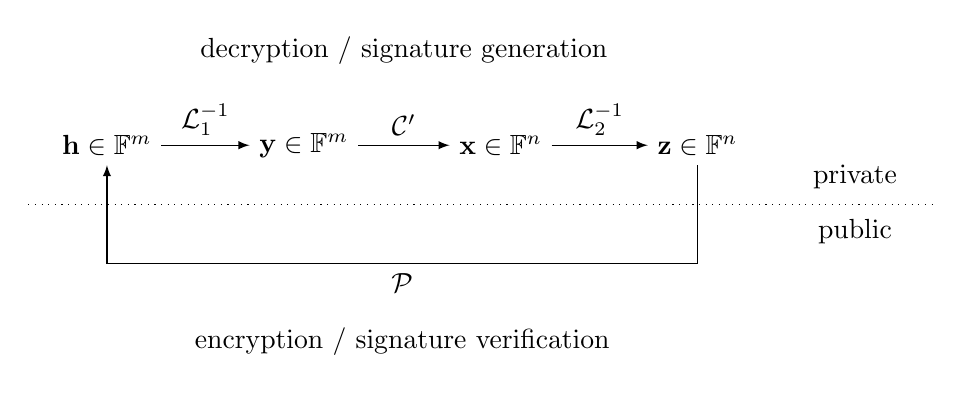
\begin{tikzpicture}
    \node (h) at (-2.5, 0) {$\mathbf{h} \in \mathbb{F}^{m}$};
    \node (y) at (0, 0) {$\mathbf{y} \in \mathbb{F}^{m}$};
    \node (x) at (2.5, 0) {$\mathbf{x} \in \mathbb{F}^{n}$};
    \node (z) at (5, 0) {$\mathbf{z} \in \mathbb{F}^{n}$};
    \draw[-latex] (h) -- (y) 
      node[midway,above] {$\mathcal{L}_{1}^{-1}$};
    \draw[-latex] (y) -- (x) 
      node[midway,above] {$\mathcal{C}'$}
      node[midway,yshift=1.2cm] {decryption / signature generation};
    \draw[-latex] (x) -- (z) 
      node[midway,above] {$\mathcal{L}_{2}^{-1}$};
    \draw[-latex] (z) -- (5, -1.5) -- (-2.5, -1.5) 
      node[midway,below] {$\mathcal{P}$} 
      node[midway,yshift=-1cm] {encryption / signature verification} -- (h);
    \draw[dotted] (-3.5, -0.75) -- (8, -0.75);
    \node at (7, -0.4) {private};
    \node at (7, -1.1) {public};
  \end{tikzpicture}
  \caption{Standard flow of operations in the bipolar
    construction.}\label{fig:bipolar}
\end{figure}

We now observe the relationship between $m$ and $n$ to understand how the bipolar construction works. The lateral maps need not be considered in this discussion due to their lack of structure. For $m \geq n$, the map $\mathcal{C}$ should be injective, to ensure that there exists a unique plaintext $\mathbf{z}$ related to each ciphertext $\mathbf{h}$, by the preimage step. In the case of $m \leq n$, one expects that $\mathcal{C}$ is surjective, such that every message $\mathbf{h}$ has a signature $\mathbf{z}$, once again by the central map preimage.

The private and public keys are respectively a $3$-tuple and its aforementioned composition, that is,
\begin{align}
  \begin{split}
    \mathsf{sk} &= (\mathcal{L}_{1}, \mathcal{C}, \mathcal{L}_{2}) 
      \in \mathsf{GL}(\mathbb{F}^{m}) \times \mathsf{MQ}(n, m) \times \mathsf{GL}(\mathbb{F}^{n}), \\
    \mathsf{pk} &= \mathcal{P} \in \mathsf{MQ}(n, m).
  \end{split}
\end{align}
The bipolar construction can be extended to work differently from the main idea given, for instance in the case of schemes that perform calculations over multiple finite fields. We invite the reader to consult~\cite[Section 2.2]{Petzoldt:201307} for a discussion of such schemes, and even ones that do not use the construction at all.

While very elegant, the bipolar construction yields a situation in which derived schemes are not exclusively based on Definition~\ref{def:posso}. There exist signature schemes constructed via the Fiat--Shamir transformation which only depend on \textsf{PoSSo} such as MQDSS~\cite{Chen:201612}, but their efficiency is lacking compared to schemes based on the bipolar construction. Consequently, a scheme using the bipolar construction is also based on some variant of the \emph{isomorphism of polynomials (IP) problem}. There are several versions of the IP problem, and we give a short definition for the variant that Oil--Vinegar schemes are based on, as introduced in~\cite{Ding:200806}.

\begin{definition}\label{def:eip}
  Let $\overline{\mathsf{MQ}}(n, m)$ be a class of structured quadratic polynomial maps and $\mathbb{U} = \mathsf{GL}(\mathbb{F}^{m}) \times \overline{\mathsf{MQ}}(n, m) \times \mathsf{GL}(\mathbb{F}^{n})$ be a set of private keys. Given a $3$-tuple $(\mathcal{L}_{1}, \mathcal{C}, \mathcal{L}_{2}) \in \mathbb{U}$ with $\mathcal{P} = \mathcal{L}_{1} \circ \mathcal{C} \circ \mathcal{L}_{2}$, finding a decomposition $\mathcal{P} = \widetilde{\mathcal{L}}_{1} \circ \widetilde{\mathcal{C}} \circ \widetilde{\mathcal{L}}_{2}$ such that $(\widetilde{\mathcal{L}}_{1}, \widetilde{\mathcal{C}}, \widetilde{\mathcal{L}}_{2}) \in \mathbb{U}$ is the \emph{extended isomorphism of polynomials (EIP) problem}.
\end{definition}

Unfortunately, the amount of information regarding the difficulty of EIP is sparse~\cite[p.~69]{Thomae:201306}, preventing complete security proofs for Oil--Vinegar schemes. This is also the case for other IP problems, so that most multivariate cryptosystems simply have \emph{ad hoc} security. A consequence of EIP is that there exist many private keys that compose a single public key~\cite{Wolf:201104}, and this has been used to attack several schemes, as seen in Section~\ref{sec:related}.

\begin{definition}
  Let $\mathbb{U}$ as per Definition~\ref{def:eip}. Given two private keys $(\mathcal{L}_{1}, \mathcal{C}, \mathcal{L}_{2}), (\widetilde{\mathcal{L}}_{1}, \widetilde{\mathcal{C}}, \widetilde{\mathcal{L}}_{2}) \in \mathbb{U}$, they are \emph{equivalent keys} if
  \begin{align}
    \mathcal{P} = \mathcal{L}_{1} \circ \mathcal{C} \circ \mathcal{L}_{2}
      = \widetilde{\mathcal{L}}_{1} \circ \widetilde{\mathcal{C}} \circ \widetilde{\mathcal{L}}_{2}.
  \end{align}
\end{definition}

\begin{definition}\label{def:sustainer}
  Given a private key $(\mathcal{L}_{1}, \mathcal{C}, \mathcal{L}_{2}) \in \mathbb{U}$, the linear transformations $\tau \in \mathsf{GL}(\mathbb{F}^{m}),\: \omega \in \mathsf{GL}(\mathbb{F}^{n})$ are \emph{sustaining transformations} if they preserve the structure of the central map, that is,
  \begin{align}
    \mathcal{P} = (\mathcal{L}_{1} \circ \tau^{-1}) \circ (\tau \circ \mathcal{C} \circ \omega) \circ (\omega^{-1} \circ \mathcal{L}_{2})
  \end{align}
  such that $\tau \circ \mathcal{C} \circ \omega \in \overline{\mathsf{MQ}}(n, m)$.
\end{definition}

This concept is further explored in the context of the schemes of Section~\ref{sec:ov}. Finally, we remark that our description of the bipolar construction is slightly different from the literature. The usual, broader description has $\mathcal{L}_{1} \in \mathsf{AGL}(\mathbb{F}^{m})$ and $\mathcal{L}_{2} \in \mathsf{AGL}(\mathbb{F}^{n})$. We recall that this is the \emph{affine group}, which is composed of matrix-vector pairs $(M, \mathbf{b})$ that encode the affine transformation $\mathbf{a} \mapsto M\mathbf{a} \bm{+} \mathbf{b}$. By setting the translation vector $\mathbf{b} = (0, \dots, 0)$, we get a linear transformation. 

However, it is argued in~\cite[Remark 3.1]{Wolf:201104} that due to the theory of equivalent keys, it is not relevant to the security of most schemes based on the bipolar construction if $\mathcal{L}_{1}$ and $\mathcal{L}_{2}$ are linear instead of affine transformations. Hence, our description of the bipolar construction is based on this technical result. Furthermore, there is independent evidence of this fact for the schemes presented in Section~\ref{sec:ov}. 

It is argued in~\cite[Lemmas 3.2, 3.10, 3.19]{Thomae:201306} that some IP problems modelled to represent Oil--Vinegar schemes are no harder to solve using linear transformations in place of affine ones. As a consequence, the polynomials in the central map must be homogeneous quadratic. Moreover, there exist works that confirm homogeneous quadratic maps and linear transformations are safe both in UOV~\cite[Section 5]{Kipnis:199808}~\cite[Section 3.1]{Braeken:200502} and Rainbow~\cite[Section 3.1]{Ding:201901}.

\section{The Oil--Vinegar trapdoor}\label{sec:ov}

In this section, we describe the classic schemes based on the Oil--Vinegar trapdoor, introduced in~\cite{Patarin:199709}. We define the Unbalanced Oil and Vinegar (UOV) signature scheme in Subsection~\ref{subsec:uov}, alongside with its multi-layer generalization Rainbow, in Subsection~\ref{subsec:rainbow}. We discuss the theory of equivalent keys for each scheme alongside their descriptions. Our definitions are based on~\cite[Chapter 3]{Ding:2006} and~\cite[Chapter 3]{Petzoldt:201307}.

\subsection{Unbalanced Oil and Vinegar signature scheme}\label{subsec:uov}

The idea of the original Oil and Vinegar signature scheme is to build the central map with two sets of variables, \emph{vinegar and oil variables}, such that the multivariate quadratic polynomials do not feature any quadratic oil terms. Thus, by choosing the values of vinegar variables, the systems become linear in the oil variables and consequently easy to solve.

\begin{definition}\label{def:oil-vinegar-poly}
  Given $v, o \in \mathbb{N}$, let $V = \{1, \dots, v\}$, $O = \{v + 1, \dots, v + o\}$ and $\mathbf{x} = (x_{1}, \dots, x_{v}, x_{v + 1}, \dots, x_{v + o})$. Given a polynomial ring $\mathbb{F}[\mathbf{x}]$, an \emph{Oil--Vinegar polynomial} is a multivariate quadratic polynomial of the form
  \begin{align}
    \sum_{i \in V} \sum_{j \in V} \alpha_{ij} x_{i} x_{j}
      + \sum_{i \in V} \sum_{j \in O} \beta_{ij} x_{i} x_{j}
      + \sum_{i \in V \cup O} \gamma_{i} x_{i}
      + \delta,
  \end{align}
  where $\alpha_{ij}, \beta_{ij}, \gamma_{i}, \delta \in \mathbb{F}$. The set of all such polynomials is defined as $\mathsf{OVP}(v, o)$.
\end{definition}

\begin{definition}
  Let $n = v + o$. A polynomial map $\mathcal{C} : \mathbb{F}^{n} \to \mathbb{F}^{o}$ consisting of $f^{(1)}, \dots, f^{(o)} \in \mathsf{OVP}(v, o)$ is an \emph{Oil--Vinegar polynomial map}. The set of all such maps is defined as $\mathsf{OV}(n, o)$. If all polynomials are homogeneous quadratic, then the respective set is $\mathsf{OVH}(v, o)$.
\end{definition}

The integers $v$ and $o$ represent the quantity of vinegar and oil variables, respectively. After the substitution of vinegar variables, the resulting system is exactly determined, with $o$ equations and $o$ variables. We remark that the first summation of Definition~\ref{def:oil-vinegar-poly} is explicitly split into cross-vinegar terms, and product of vinegar and oil terms, to emphasize that there do not exist cross-oil terms. An intuitive visualization of this structure is given below.

\begin{definition}
  Given a homogeneous quadratic Oil--Vinegar polynomial $f^{(i)} \in \mathsf{OVH}(v, o)$, its matrix representation is
  \begin{align}
    \widetilde{M}(f^{(i)}) =
    \begin{bmatrix}
      \star_{v \times v} & \star_{v \times o} \\
      \star_{o \times v} & \mathbf{0}_{o \times o} \\
    \end{bmatrix}.
  \end{align}
\end{definition}
We are now ready to describe the Oil--Vinegar signature scheme.

\subsubsection{Key generation.}

Since Oil--Vinegar schemes are based on the bipolar construction, the private key is composed of a central map $\mathcal{C}$ and a linear transformation $\mathcal{L}_{2}$ to hide its structure. We remark that the linear transformation $\mathcal{L}_{1}$ is always $\mathsf{id}$, since it simply performs a permutation of the coefficients in the central map~\cite[p.~71]{Thomae:201306} and is not relevant to the security of the scheme. Hence, we do not consider $\mathcal{L}_{1}$ to be part of the private key. Then, let
\begin{align}\label{eq:sk-uov}
  \mathsf{sk} = (\mathcal{C}, \mathcal{L}_{2})
    \random \mathsf{OV}(n, o) \times \mathsf{GL}(\mathbb{F}^{n}).
\end{align}

In the case of $\mathcal{C}$, the random choice amounts to picking all coefficients of the polynomials at random. For $\mathcal{L}_{2}$, a new matrix with random coefficients is generated until it is invertible. As discussed in Section~\ref{sec:mult}, we choose the lateral maps to be linear transformations, since it is proven that this also does not affect the security of Oil--Vinegar schemes~\cite[Section 3.1]{Braeken:200502}. The same fact holds for homogeneous quadratic Oil--Vinegar polynomials. Let $\mathcal{P} = \mathcal{C} \circ \mathcal{L}_{2}$ and
\begin{align}\label{eq:pk-uov}
  \mathsf{pk} = \mathcal{P} \in \mathsf{MQ}(n, o).
\end{align}

\subsubsection{Signature generation.}

Consider a cryptographic hash function $\mathcal{H} : \{0, 1\}^{*} \to \mathbb{F}^{o}$, any message $M \in \{0, 1\}^{*}$, and obtain the message digest $\mathbf{h} = \mathcal{H}(M)$. The Oil--Vinegar trapdoor is built to allow the signer to randomly choose vinegar variables $x_{1}, \dots, x_{v}$ such that a preimage of the message digest can be obtained, by solving for the remaining oil variables $\mathcal{C}(x_{1}, \dots, x_{v}, x_{v + 1}, \dots, x_{v + o}) = \mathbf{h}$. 

To sign a message, one chooses $(x_{1}, \dots, x_{v}) \random \mathbb{F}^{v}$, substitutes these values into $\mathcal{C}(\mathbf{x}) = \mathbf{h}$ and solves the resulting linear system with, for instance, Gaussian elimination, obtaining the remaining values of $\mathbf{x}$. Usual parameters for Oil--Vinegar schemes are small enough, as per Subsection~\ref{sec:exp}, such that special methods for solving linear systems are not needed. 

If the linear system is inconsistent due to a bad choice of vinegar variables, new ones are simply picked again. This happens with a very low probability, as seen in Subsection~\ref{subsec:invert}. Then, the signature is the result of the inverse linear transformation applied to the preimage. In other words, $\mathbf{z} = \mathcal{L}_{2}^{-1}(\mathbf{x})$.

\subsubsection{Signature verification.}

To verify a signature, compute $\mathbf{h'} = \mathcal{P}(\mathbf{z})$. If $\mathbf{h} = \mathbf{h'}$, then the signature is valid, and otherwise invalid.

The balanced Oil--Vinegar scheme occurs when $v = o$. However, it was found to be insecure shortly after its proposal~\cite{Kipnis:199808}. We discuss this attack in Chapter~\ref{ch:attack}. In the following year, the UOV variant with $v = 2o$ was proposed as a secure variant~\cite{Kipnis:199904}, and no security weaknesses are known to the date of writing, if the correct choice of parameters is performed. An instance of UOV is denoted by $\mathsf{UOV}(\mathbb{F}, v, o)$. 

The size of a private key is the number of elements in $\psi(\mathcal{L}_{2})$, added to the count of all valid monomial combinations in $\mathcal{C}$. In other words,
\begin{align}
  \#\mathsf{sk} = \underbrace{o \cdot \left( \frac{v \cdot (v + 1)}{2} + v \cdot o + v + o + 1 \right)}_{\mathcal{C}} \;
    + \; \underbrace{n^{2}}_{\mathcal{L}_{2}}
\end{align}
field elements. The size of a public key is the number of coefficients of $o$ polynomials in the ring $\mathbb{F}[x_{1}, \dots, x_{n}]$, which is known to be $\binom{n + d}{d}$ for the degree $d \in \mathbb{N}$. Since Oil--Vinegar polynomials are quadratic, we have $d = 2$, and hence
\begin{align}
  \#\mathsf{pk} = o \cdot \frac{(n + 1) \cdot (n + 2)}{2}
\end{align}
field elements. We note that if the Oil--Vinegar polynomials are homogeneous quadratic, then the private key size decreases by $o \cdot (v + o + 1)$ elements, and the public key size decreases by $o \cdot (n + 1)$ elements.

\subsubsection{Equivalent keys.}

We recall that there exists a specific form of sustainers of Definition~\ref{def:sustainer} for each scheme. In the case of UOV, these mappings are given in~\cite[Section 4.3]{Wolf:201104}. We follow the notation of~\cite{Petzoldt:201307}.

\begin{theorem}[{\cite[Theorem 4.15]{Wolf:201104}}]
  Given a private key $(\mathcal{C}, \mathcal{L}_{2}) \in \mathsf{OV}(n, o) \times \mathsf{GL}(\mathbb{F}^{n})$ and $\omega \in \mathsf{GL}(\mathbb{F}^{n})$ such that
  \begin{align}
    \psi(\omega) =
    \begin{bmatrix}
      \omega_{v \times v}^{(1)} & \mathbf{0}_{v \times o} \\
      \omega_{o \times v}^{(2)} & \omega_{o \times o}^{(3)} \\
    \end{bmatrix}
  \end{align}
  with $\omega^{(1)} \in \mathsf{GL}_{v}(\mathbb{F})$ and $\omega^{(3)} \in \mathsf{GL}_{o}(\mathbb{F})$, then $(\mathcal{C} \circ \omega, \omega^{-1} \circ \mathcal{L}_{2})$ is an equivalent private key.
\end{theorem}

We remark that $\psi(\omega^{-1})$ has the same form as $\omega$ due to the restrictions on $\omega^{(1)}$ and $\omega^{(3)}$, that is,
\begin{align}
  \psi(\omega^{-1}) =
  \begin{bmatrix}
    (\omega^{(1)})^{-1}                                                 & \mathbf{0}_{v \times o}   \\
    -(\omega^{(3)})^{-1} \cdot \omega^{(2)} \cdot (\omega^{(1)})^{-1}   & (\omega^{(3)})^{-1}       \\
  \end{bmatrix},
\end{align}
where we remove the sub-indices that indicate the dimension of the block matrices to improve readability. It is a direct consequence of this theorem that there exist at least as many equivalent keys as possible choices for $\omega$. This redundancy may be cast away by observing the shape of $\omega^{-1} \circ \mathcal{L}_{2}$ and only selecting lateral maps with this structure.

\begin{theorem}[{\cite[Theorem 2]{Beullens:201706}}]
  Given a private key $(\mathcal{C}, \mathcal{L}_{2}) \in \mathsf{OV}(n, o) \times \mathsf{GL}(\mathbb{F}^{n})$ and $\omega \in \mathsf{GL}(\mathbb{F}^{n})$ such that
  \begin{align}
    \psi(\mathcal{L}_{2}) =
    \begin{bmatrix}
      \mathcal{L}_{2}^{(1)} & \mathcal{L}_{2}^{(2)} \\
      \mathcal{L}_{2}^{(3)} & \mathcal{L}_{2}^{(4)} \\
    \end{bmatrix},\;
    \psi(\omega) =
    \begin{bmatrix}
      \mathcal{L}_{2}^{(1)} & \mathbf{0}_{v \times o} \\
      \mathcal{L}_{2}^{(3)} & \mathcal{L}_{2}^{(4)} -\mathcal{L}_{2}^{(3)} \cdot (\mathcal{L}_{2}^{(1)})^{-1} \cdot \mathcal{L}_{2}^{(2)} \\
    \end{bmatrix}
  \end{align}
  and $\mathcal{L}_{2}^{(1)} \in \mathsf{GL}_{v}(\mathbb{F})$, then
  \begin{align}
    \psi(\omega^{-1} \circ \mathcal{L}_{2}) = \begin{bmatrix}
      \mathbf{I}_{v} & (\mathcal{L}_{2}^{(1)})^{-1} \cdot \mathcal{L}_{2}^{(2)} \\
      \mathbf{0}_{o \times v} & \mathbf{I}_{o} \\
    \end{bmatrix}.
  \end{align}
\end{theorem}

Then, as long as $\mathcal{L}_{2}^{(1)}$ is invertible, there exists an equivalent key for UOV. This happens with overwhelming probability as per Subsection~\ref{subsec:invert}. Hence, one may simply choose $\widetilde{\mathcal{L}}_{2} \in \mathsf{GL}(\mathbb{F}^{n})$ such that
\begin{align}
  \psi(\widetilde{\mathcal{L}}_{2}) =
  \begin{bmatrix}
    \mathbf{I}_{v}          & \star_{v \times o} \\
    \mathbf{0}_{o \times v} & \mathbf{I}_{o} \\
  \end{bmatrix}
\end{align}
and obtain a reduction in the private key size of a factor $\frac{n^{2}}{v o}$.

\subsection{Rainbow signature scheme}\label{subsec:rainbow}

The Rainbow signature scheme, originally defined in~\cite{Ding:200506} and a finalist of the NIST standardization process~\cite[Section~3.20]{Alagic:202007}, is a generalized version of UOV that reduces the length of keys and signatures. This is achieved due to the combination of several smaller ``oil and vinegar'' layers, that are combined to create a ``rainbow''.

Consider a finite field $\mathbb{F}$ and $u, n \in \mathbb{N}$ where $u \leq n$. Choose a sequence of integers $v_{1}, \dots, v_{u}$ such that $0 = v_{0} < v_{1} < \cdots < v_{u} < v_{u + 1} = n$. Take the usual set $V = \{1, \dots, n\}$ and, for the range $1 \leq l \leq u$, define vinegar variables as $V_{\ell} = \{1, \dots, v_{\ell}\}$ and oil variables as $O_{\ell} = \{v_{\ell} + 1, \dots, v_{\ell + 1}\}$. We note that $V_{1} \subset \dots \subset V_{u + 1} = V$ and $O_{\ell} = V_{\ell + 1} \setminus V_{\ell}$. Let $o_{\ell} = |O_{\ell}|$ and $m = n - v_{1}$. Now, we define $u$ vector spaces spanned by quadratic Oil--Vinegar polynomials of the form $\mathsf{OV}(v_{\ell}, o_{\ell})$, that is,
\begin{align}\label{eq:oil-vinegar-space}
  \sum_{i \in V_{\ell}} \sum_{j \in V_{\ell}} \alpha_{ij} x_{i} x_{j}
    + \sum_{i \in V_{\ell}} \sum_{j \in O_{\ell}} \beta_{ij} x_{i} x_{j}
    + \sum_{i \in V_{\ell} \cup O_{\ell}} \gamma_{i} x_{i} + \delta,
\end{align}
where $\alpha_{ij}, \beta_{ij}, \gamma_{i}, \delta \in \mathbb{F}$. We define $\mathsf{RB}(v_{1}, o_{1}, \dots, o_{u}) = \mathsf{OV}(v_{1}, o_{1}) \times \cdots \times \mathsf{OV}(v_{u}, o_{u})$. We are now ready to describe the Rainbow signature scheme.

\subsubsection{Key generation.}

In the case of Rainbow, all three maps are needed to securely hide the structure of the central map. Therefore,
\begin{align}\label{eq:sk-rainbow}
  \mathsf{sk} = (\mathcal{L}_{1}, \mathcal{C}, \mathcal{L}_{2}) 
    \random \mathsf{GL}(\mathbb{F}^{m}) \times \mathsf{RB}(v_{1}, o_{1}, \dots, o_{u}) \times \mathsf{GL}(\mathbb{F}^{n}).
\end{align}

For the central map $\mathcal{C}$, the random choice is equivalent to randomly choosing polynomial systems from each $\mathsf{OV}(v_{\ell}, o_{\ell})$ with $1 \leq l \leq u$, analogous to multiple UOV systems. The linear transformations are random invertible matrices. Since each sequence of vinegar variables in a layer contains all oil and vinegar variables from the previous layer, this allows for the correct preimage calculation of $\mathcal{C}$. Let $\mathcal{P} = \mathcal{L}_{1} \circ \mathcal{C} \circ \mathcal{L}_{2}$ and
\begin{align}\label{eq:pk-rainbow}
  \mathsf{pk} &= \mathcal{P} \in \mathsf{MQ}(n, m).
\end{align}
For example, in the case of $u = 2$ and $1 \leq i \leq m$, the matrix representation of a homogeneous quadratic $\mathcal{C}$ is
\begin{align}
  \widetilde{M}(f^{(i)}) =
  \begin{dcases}
    \begin{bmatrix}
      \star_{v_{1} \times v_{1}}      & \star_{v_{1} \times o_{1}}      & \mathbf{0}_{v_{1} \times o_{2}} \\
      \star_{o_{1} \times v_{1}}      & \mathbf{0}_{o_{1} \times o_{1}} & \mathbf{0}_{o_{1} \times o_{2}} \\
      \mathbf{0}_{o_{2} \times v_{1}} & \mathbf{0}_{o_{2} \times o_{1}} & \mathbf{0}_{o_{2} \times o_{2}} \\
    \end{bmatrix} & \text{for } f^{(1)}, \dots, f^{(o_{1})} \in \mathcal{C}, \\
    \begin{bmatrix}
      \star_{v_{1} \times v_{1}}      & \star_{v_{1} \times o_{1}}      & \star_{v_{1} \times o_{2}} \\
      \star_{o_{1} \times v_{1}}      & \star_{o_{1} \times o_{1}}      & \mathbf{0}_{o_{1} \times o_{2}} \\
      \star_{o_{2} \times v_{1}}      & \mathbf{0}_{o_{2} \times o_{1}} & \mathbf{0}_{o_{2} \times o_{2}} \\
    \end{bmatrix} & \text{for } f^{(o_{1} + 1)}, \dots, f^{(o_{2})} \in \mathcal{C}.
  \end{dcases}
\end{align}

\subsubsection{Signature generation.}

Consider a cryptographic hash function $\mathcal{H} : \{0, 1\}^{*} \to \mathbb{F}^{m}$, any message $M \in \{0, 1\}^{*}$, and obtain the message digest $\mathbf{h} = \mathcal{H}(M)$. Compute $\mathbf{y} = \mathcal{L}_{1}^{-1}(\mathbf{h})$. To obtain the preimage $\mathcal{C}(\mathbf{x}) = \mathbf{y}$, every layer must be inverted recursively. One chooses $(x_{1}, \dots, x_{v_{1}}) \random \mathbb{F}^{v_{1}}$ and substitutes the values into the first layer, or in other words, the first system of $o_{1}$ polynomials. This brings forth a system of $o_{1}$ linear equations in $x_{v_{1} + 1}, \dots, x_{v_{2}}$. It can be solved with an algorithm such as Gaussian elimination. If the system does not have a solution, new vinegar variables $x_{1}, \dots, x_{v_{1}}$ have to be chosen. These solutions can then be substituted into the next layer, which creates a system of $o_{2}$ linear equations, that can be solved analogously. This procedure is repeated until all layers are solved. Finally, we compute $\mathbf{z} = \mathcal{L}_{2}^{-1}(\mathbf{x})$.

\subsubsection{Signature verification.}

To verify a signature, compute $\mathbf{h'} = \mathcal{P}(\mathbf{z})$. If $\mathbf{h} = \mathbf{h'}$, then the signature is valid, and otherwise invalid.

The remarks about UOV regarding the size of parameters, chances of failure in the central map preimage calculation and lack of security weaknesses are maintained in the case of Rainbow. An instance of Rainbow is denoted by $\mathsf{Rainbow}(\mathbb{F}, v_{1}, o_{1}, \dots, o_{u})$, with usually $u = 2$ for efficiency reasons. We note that when $u = 1$, we get the UOV scheme.

Measured in field elements, the size of a private key is the number of elements in $\psi(\mathcal{L}_{1})$ and $\psi(\mathcal{L}_{2})$, added to the count of all valid monomial combinations from each layer of Oil--Vinegar polynomials as per Equation (\ref{eq:oil-vinegar-space}). In other words,
\begin{align}\label{eq:sk-size-rainbow}
  \#\mathsf{sk} = \underbrace{m^{2}}_{\mathcal{L}_{1}} 
    + \underbrace{\sum_{k = 1}^{u} o_{k} \cdot \left( \frac{v_{k} \cdot (v_{k} + 1)}{2} + v_{k} \cdot o_{k} + v_{k} + o_{k} + 1 \right)}_{\mathcal{C}}
    + \underbrace{n^{2}}_{\mathcal{L}_{2}}.
\end{align}
The size of a public key is similar to the UOV case, and thus we have
\begin{align}
  \#\mathsf{pk} = m \cdot \frac{(n + 1) \cdot (n + 2)}{2}
\end{align}
field elements. If polynomials are homogeneous quadratic, then the private key size decreases by $\sum_{k = 1}^{u} o_{k} \cdot (v_{k} + o_{k} + 1)$ elements, and the public key size decreases by $m \cdot (n + 1)$ elements.

\subsubsection{Equivalent keys.}

As a generalization of UOV, there exist equivalent keys in Rainbow using a similar rationale. The theory is developed in~\cite[Section 4.4]{Wolf:201104} for STS, which as previously mentioned is a special sparse case of Rainbow. It is argued in~\cite{Petzoldt:201307} that the strategy is also suitable for Rainbow.

\begin{theorem}[{\cite[Theorem 4.17]{Wolf:201104}}]
  Without loss of generality, consider a private key $(\mathcal{L}_{1}, \mathcal{C}, \mathcal{L}_{2}) \in \mathsf{GL}(\mathbb{F}^{m}) \times \mathsf{RB}(v_{1}, o_{1}, \dots, o_{u}) \times \mathsf{GL}(\mathbb{F}^{n})$ with $u = 2$. Given $\tau \in \mathsf{GL}(\mathbb{F}^{m})$ and $\omega \in \mathsf{GL}(\mathbb{F}^{n})$ such that
  \begin{align}
    \psi(\tau) =
    \begin{bmatrix}
      \tau_{o_{1} \times o_{1}}^{(1)} & \mathbf{0}_{o_{1} \times o_{2}} \\
      \tau_{o_{2} \times o_{1}}^{(2)} & \tau_{o_{2} \times o_{2}}^{(3)} \\
    \end{bmatrix},\;
    \psi(\omega) =
    \begin{bmatrix}
      \omega_{v_{1} \times v_{1}}^{(1)} & \mathbf{0}_{v_{1} \times o_{1}}   & \mathbf{0}_{v_{1} \times o_{2}} \\
      \omega_{o_{1} \times v_{1}}^{(2)} & \omega_{o_{1} \times o_{1}}^{(3)} & \mathbf{0}_{o_{1} \times o_{2}} \\
      \omega_{o_{2} \times v_{1}}^{(4)} & \omega_{o_{2} \times o_{1}}^{(5)} & \omega_{o_{2} \times o_{2}}^{(6)} \\
    \end{bmatrix},
  \end{align}
  $\omega^{(1)} \in \mathsf{GL}_{v_{1}}(\mathbb{F}),\; \tau^{(1)}, \omega^{(3)} \in \mathsf{GL}_{o_{1}}(\mathbb{F})$ and $\tau^{(3)}, \omega^{(6)} \in \mathsf{GL}_{o_{2}}(\mathbb{F})$, then $(\mathcal{L}_{1} \circ \tau^{-1}, \tau \circ \mathcal{C} \circ \omega, \omega^{-1} \circ \mathcal{L}_{2})$ is an equivalent private key.
\end{theorem}

The linear transformations $\tau^{-1}$ and $\omega^{-1}$ maintain their forms by a similar block inverse calculation, as seen below. We use a compact notation to represent operations between inner block matrices for easier reading. For example, $-(\tau^{(3)})^{-1} \cdot \tau^{(2)} \cdot (\tau^{(1)})^{-1}$ is denoted as $\tau^{(-3^{-1} \cdot 2 \cdot 1^{-1})}$. Then,
\begin{align}
  \begin{split}
    \psi(\tau^{-1}) &=
    \begin{bmatrix}
      (\tau^{(1)})^{-1} & \mathbf{0}_{o_{1} \times o_{2}} \\
      \tau^{(-3^{-1} \cdot 2 \cdot 1^{-1})} & (\tau^{(3)})^{-1} \\
    \end{bmatrix}, \\
    \psi(\omega^{-1}) &=
    \begin{bmatrix}
      (\omega^{(1)})^{-1} & \mathbf{0}_{v_{1} \times o_{1}} & \mathbf{0}_{v_{1} \times o_{2}} \\
      \omega^{(-3^{-1} \cdot 2 \cdot 1^{-1})} & (\omega^{(3)})^{-1} & \mathbf{0}_{o_{1} \times o_{2}} \\
      % TODO
      {\color{red} \star} & \omega^{(-6^{-1} \cdot 5 \cdot 3^{-1})} & (\omega^{(6)})^{-1} \\
    \end{bmatrix}.
  \end{split}
\end{align}
The redundancy is removed by the same rationale of UOV, observing the shape of the lateral maps in the equivalent key.

\begin{theorem}[{\cite[Theorem 3.6]{Petzoldt:201307}}]\label{thm:eq-keys-rainbow}
  Without loss of generality, consider a private key $(\mathcal{L}_{1}, \mathcal{C}, \mathcal{L}_{2}) \in \mathsf{GL}(\mathbb{F}^{m}) \times \mathsf{RB}(v_{1}, o_{1}, \dots, o_{u}) \times \mathsf{GL}(\mathbb{F}^{n})$ with $u = 2$, such that
  \begin{align}
    \psi(\mathcal{L}_{1}) =
    \begin{bmatrix}
      \mathcal{L}_{1}^{(1)} & \mathcal{L}_{1}^{(2)} \\
      \mathcal{L}_{1}^{(3)} & \mathcal{L}_{1}^{(4)} \\
    \end{bmatrix} \text{and }
    \psi(\mathcal{L}_{2}) =
    \begin{bmatrix}
      \mathcal{L}_{2}^{(1)} & \mathcal{L}_{2}^{(2)} & \mathcal{L}_{2}^{(3)} \\
      \mathcal{L}_{2}^{(4)} & \mathcal{L}_{2}^{(5)} & \mathcal{L}_{2}^{(6)} \\
      \mathcal{L}_{2}^{(7)} & \mathcal{L}_{2}^{(8)} & \mathcal{L}_{2}^{(9)} \\
    \end{bmatrix}.
  \end{align}
  \begin{enumerate}
    \item Given $\tau \in \mathsf{GL}(\mathbb{F}^{m})$ such that
    \begin{align}
      \psi(\tau) =
      \begin{bmatrix}
        \mathcal{L}_{1}^{(1 - 2 \cdot 4^{-1} \cdot 3)} & \mathbf{0}_{o_{1} \times o_{2}} \\
        \mathcal{L}_{1}^{(3)} & \mathcal{L}_{1}^{(4)} \\
      \end{bmatrix}
    \end{align}
    and $\mathcal{L}_{1}^{(4)} \in \mathsf{GL}_{o_{2}}(\mathbb{F})$, then
    \begin{align}
      \psi(\mathcal{L}_{1} \circ \tau^{-1}) =
      \begin{bmatrix}
        \mathbf{I}_{o_{1}} & \mathcal{L}_{1}^{(2 \cdot 4^{-1})} \\
        \mathbf{0}_{o_{2} \times o_{1}} & \mathbf{I}_{o_{2}} \\
      \end{bmatrix}.
    \end{align}
    \item Given $\omega \in \mathsf{GL}(\mathbb{F}^{n})$ such that
    \begin{align}
      \begin{split}
        \psi(\omega) &=
        \begin{bmatrix}
          \mathcal{L}_{2}^{(1)} & \mathbf{0}_{v_{1} \times o_{1}} & \mathbf{0}_{v_{1} \times o_{2}} \\
          \mathcal{L}_{2}^{(4)} & \mathcal{L}_{2}^{(5 - 4 \cdot 1^{-1} \cdot 2)} & \mathbf{0}_{o_{1} \times o_{2}} \\
          \mathcal{L}_{2}^{(7)} & \mathcal{L}_{2}^{(8 - 7 \cdot 1^{-1} \cdot 2)} & \omega^{(6)} \\
        \end{bmatrix}, \\
        \omega^{(6)} &=
        \begin{multlined}[t]
          \mathcal{L}_{2}^{((9 - 7 \cdot 1^{-1} \cdot 3) -(8 - 7 \cdot 1^{-1} \cdot 2) \cdot (5 - 4 \cdot 1^{-1} \cdot 2)^{-1} \cdot (6 - 4 \cdot 1^{-1} \cdot 3))}
        \end{multlined}
      \end{split}
    \end{align}
    with $\mathcal{L}_{2}^{(1)} \in \mathsf{GL}_{v_{1}}(\mathbb{F})$ and $\omega^{(3)} \in \mathsf{GL}_{o_{1}}(\mathbb{F})$, then
    \begin{align}
      \psi(\omega^{-1} \circ \mathcal{L}_{2}) =
      \begin{bmatrix}
        \mathbf{I}_{v_{1}} & \mathcal{L}_{2}^{(-1 \cdot 2)} & \mathcal{L}_{2}^{(-1 \cdot 3)} \\
        \mathbf{0}_{o_{1} \times v_{1}} & \mathbf{I}_{o_{1}} & (\omega^{(3)})^{-1} \cdot \mathcal{L}_{2}^{(6 - 4 \cdot 1^{-1} \cdot 3)} \\
        \mathbf{0}_{o_{2} \times v_{1}} & \mathbf{0}_{o_{2} \times o_{1}} & \mathbf{I}_{o_{2}} \\
      \end{bmatrix}.
    \end{align}
  \end{enumerate}
\end{theorem}

If $\mathcal{L}_{2}^{(1)}$ and $\omega^{(3)}$ are invertible, which once again happens with overwhelming probability, then there exists an equivalent key for Rainbow with $\widetilde{\mathcal{L}}_{1} \in \mathsf{GL}(\mathbb{F}^{m})$ and $\widetilde{\mathcal{L}}_{2} \in \mathsf{GL}(\mathbb{F}^{n})$ such that
\begin{align}
  \psi(\widetilde{\mathcal{L}}_{1}) =
  \begin{bmatrix}
    \mathbf{I}_{o_{1}} & \star_{o_{1} \times o_{2}} \\
    \mathbf{0}_{o_{2} \times o_{1}} & \mathbf{I}_{o_{2}} \\
  \end{bmatrix},\;
  \psi(\widetilde{\mathcal{L}}_{2}) =
  \begin{bmatrix}
    \mathbf{I}_{v_{1}} & \star_{v_{1} \times o_{1}} & \star_{v_{1} \times o_{2}} \\
    \mathbf{0}_{o_{1} \times v_{1}} & \mathbf{I}_{o_{1}} & \star_{o_{1} \times o_{2}} \\
    \mathbf{0}_{o_{2} \times v_{1}} & \mathbf{0}_{o_{2} \times o_{1}} & \mathbf{I}_{o_{2}} \\
  \end{bmatrix}.
\end{align}
The private key size is consequently reduced by a factor of $\frac{m^{2}}{o_{1} o_{2}} + \frac{n^{2}}{v_{1} o_{1} + v_{2} o_{2}}$.

There exists a generalization of the theory of equivalent keys, developed in~\cite{Thomae:201306}, called \emph{good keys}. It is the result of cryptanalytic developments that targeted a specific variant of Rainbow, which claimed to reduce private keys, with the intent of proving it insecure~\cite{Thomae:201207}. A particular consequence of the theory underlying this attack is that good keys may be used to further reduce private keys, through distinct linear transformations $\tau$ and $\omega$. 

More precisely, there exist several quadratic terms in the central map $\mathcal{C}$ that do not contribute to the security of the scheme, as seen in Section~\ref{subsec:linear}. The structure of the lateral maps in the context of good keys is depicted in~\cite[Figure 3]{Shim:202001}. Specifically, for $u = 2$, $\psi(\widetilde{\mathcal{L}}_{1})$ is $\mathbf{I}_{m}$, except for the last $o_{2}$ values of the $o_{1}$-th row, which are arbitrary. Analogously, $\psi(\widetilde{\mathcal{L}}_{2})$ is $\mathbf{I}_{n}$, except for the arbitrary first $v_{2}$ values of its last column. We hereafter follow the more common usage of equivalent keys in the literature, but we encourage further research on the reduction of private keys using good keys.

\chapter{New approach to reduce private keys}\label{ch:eta}

We observe that the reuse of vinegar variables in the signature generation step of the Rainbow scheme leads to a shorter representation of its central map, and thus, of the entire private key. We analyze the security implications of this strategy and present a set of modifications to the Rainbow scheme, enabling a reduction in private key sizes of up to $85\%$ with secure parameters. Additionally, this framework can be applied on top of already existing schemes that shorten either private or public keys, spawning derivatives that reduce the total key pair size by a factor of 3.5. 

\emph{The contents of this chapter are an extended version of~\cite{Zambonin:201907}.} In Section~\ref{sec:mod}, we give a formal description of our modifications, alongside with a security analysis taking into account current cryptanalytic methods for Rainbow. In Section~\ref{sec:stats}, we argue that no change of parameters is needed to maintain performance and randomness when creating signatures. In Section~\ref{sec:exp}, we measure how our modifications behave when applied to current sets of parameters for Rainbow-like schemes.

\section{Modifications to the original scheme}\label{sec:mod}

Our approach consists of modifications to the key and signature generation steps of Rainbow-like signature schemes. We propose to reuse the first set of vinegar variables for several signatures and replace these only when necessary. In other words, situations where the central map cannot be inverted and creating a signature would fail. By locking such variables and substituting them on the central map $\mathcal{C}$ early in the key generation algorithm, we create a $\overline{\mathcal{C}}$ map linear in $v_{1}$, thus reducing storage requirements. 

We recall that, as per Subsection~\ref{subsec:priv}, most variants that shorten private keys are structural in nature. Hence, the key space is limited by some heuristic with the intent of producing a compact private key. Moreover, the main approach to reduce public keys~\cite{Petzoldt:201307} prevents alterations to the private key, since it indirectly generates $\mathcal{C}$ from a partial public key through linear relations between the maps. 

Alternatively, our proposal does not modify the underlying structure of the key pair, but rather of the central map preimages, and consequently of the signatures. We thus present three general methods based on different techniques that shorten private keys in all Rainbow-like schemes. We collectively denote these by Rainbow-$\eta$, as an easy way to refer to the general method, and use the same definitions as in Subsection~\ref{subsec:rainbow}, further denoting the vinegar variables for the first layer as $\widetilde{V}_{1} = (x_{1}, \dots, x_{v_{1}})$.

\subsection{Usage of a seed}

We use the fact that a PRNG has the ability to recreate the same sequence of numbers given a seed. The choice of such a generator is outside the scope of our work, and we assume that a cryptographically secure PRNG is chosen. This approach is similar to~\cite{Shim:201512}, but it is not as costly, since the private key does not need to be recreated before every signature generation. It is best suited to environments in which an efficient generator is previously supplied. We are not aware of any Rainbow variants that disallow this practice. We denote this variant as Rainbow-$\eta_{1}$.

\subsubsection{Key generation.}

We bound the creation of the key pair to a seed $\mathbf{S} \in \mathbb{N}_{0}$. Thus, $\mathcal{L}_{1}$, $\mathcal{C}$ and $\mathcal{L}_{2}$ are generated through the target scheme key generation algorithm, seeded by $\mathbf{S}$. The composition $\mathcal{P} = \mathcal{L}_{1} \circ \mathcal{C} \circ \mathcal{L}_{2}$ must be obtained before the substitution of the vinegar variables such that it does not need to be recreated. We then choose $\widetilde{V}_{1} \random \mathbb{F}^{v_{1}}$ and substitute these into $\mathcal{C}$, giving $\overline{\mathcal{C}} \in \mathsf{RB}(v_{2}, o_{2}, \dots, o_{u})$. Finally,
\begin{align}
  \begin{split}
    \mathsf{sk}^{\eta_{1}} &= (\mathbf{S}, \widetilde{V}_{1}, \mathcal{L}_{1}, \overline{\mathcal{C}}, \mathcal{L}_{2}), \\
    \mathsf{pk}^{\eta_{1}} &= \mathcal{P}.
  \end{split}
\end{align}

\subsubsection{Signature generation.}

This step does not change significantly from the original scheme. Consider a message $M$ and obtain its digest $\mathbf{h} = \mathcal{H}(M)$. Compute $\mathbf{y} = \mathcal{L}_{1}^{-1}(\mathbf{h})$. The preimage $\overline{\mathcal{C}}(\mathbf{x}) = \mathbf{y}$ already has its first $v_{1}$ elements set in the form of $\widetilde{V}_{1}$. The rest are obtained by recursively solving the remaining linear systems arising from the first layer. In the rare case that a failure occurs in the central map inversion algorithm, we invoke the key generation step with $\mathbf{S}$ to obtain $\mathcal{C}$, choose other values for $\widetilde{V}_{1}$ and create a different $\overline{\mathcal{C}}$. Finally, compute $\mathbf{z} = \mathcal{L}_{2}^{-1}(\mathbf{x})$.

\subsubsection{Signature verification.}

This step does not change. To verify a signature, compute $\mathbf{h'} = \mathcal{P}(\mathbf{z})$. If $\mathbf{h} = \mathbf{h'}$, then the signature is valid, and otherwise invalid.

\subsection{Linear relations of Petzoldt}\label{subsec:linear}

This approach is based on the fact that a private key owner is able to recover the original central map through the possession of the lateral maps and the public key. We make use of the linear relations first introduced in~\cite{Petzoldt:201006} and applied in the definition of the well-known CyclicRainbow scheme. We denote this variant as Rainbow-$\eta_{2}$. A brief explanation of the relations is given below, with the full rationale available in~\cite[Chapter 7]{Petzoldt:201307}. 

Consider the key pair of a UOV signature scheme as described in Equations (\ref{eq:sk-uov}) and (\ref{eq:pk-uov}). It is known that quadratic terms do not mix with linear and constant terms in the case of Oil--Vinegar signature schemes, and thus we refer only to the quadratic part of any polynomial systems in our description. Let the quadratic part of the $k$-th polynomial $c^{(k)} \in \mathcal{C},\; 1 \leq k \leq m$, represented by Definition~\ref{def:oil-vinegar-poly}, be denoted as
\begin{align}
  \widetilde{c}^{(k)} = \sum_{i = 1}^{n} \sum_{j = i}^{n} \alpha_{ij}^{(k)} x_{i} x_{j}.
\end{align}
Further, we analogously denote the quadratic part of $h^{(k)} \in \mathcal{P}$ as
\begin{align}\label{eq:quad-part-uov-pk}
  \widetilde{h}^{(k)} = \sum_{i = 1}^{n} \sum_{j = i}^{n} \nu_{ij}^{(k)} x_{i} x_{j}.
\end{align}
Let the elements of $\psi(\mathcal{L}_{2})$ be denoted as $d_{ij}, 1 \leq i, j \leq n$. We recall that the function composition $\mathcal{P} = \mathcal{C} \circ \mathcal{L}_{2}$ can be represented as a series of matrix multiplication operations. For instance, Equation (\ref{eq:quad-part-uov-pk}) may be rewritten as
\begin{align}\label{eq:quad-part-uov-pk-subst}
  \widetilde{h}^{(k)} = \sum_{i = 1}^{n} \sum_{j = i}^{n} \left( \alpha_{ij}^{(k)} \sum_{r = 1}^{n} d_{ri} x_{r} \sum_{s = 1}^{n} d_{sj} x_{s} \right).
\end{align}
Focusing on the inner summation, we can represent the matrix multiplication by $\psi(\mathcal{L}_{2})$ in a compact way by letting
\begin{align}
  d_{rs}^{(ij)} =
  \begin{dcases}
    d_{ri} \cdot d_{rj}                         & \text{if } r = s, \\
    d_{ri} \cdot d_{sj} + d_{si} \cdot d_{rj}   & \text{otherwise},
  \end{dcases}
\end{align}
allowing the rewrite of Equation (\ref{eq:quad-part-uov-pk-subst}) as
\begin{align}
  \widetilde{h}^{(k)} = \sum_{i = 1}^{n} \sum_{j = i}^{n} \left( \alpha_{ij}^{(k)} \sum_{r = 1}^{n} \sum_{s = 1}^{n} d_{rs}^{(ij)} x_{r} x_{s} \right).
\end{align}
If we recall Equation (\ref{eq:quad-part-uov-pk}), the coefficient associated with the monomial $x_{i} x_{j}$ of the public key is thus exactly
\begin{align}\label{eq:sk-pk-linear-rel}
  \nu_{ij}^{(k)} = \sum_{i = 1}^{n} \sum_{j = i}^{n} \alpha_{ij}^{(k)} \sum_{r = 1}^{n} \sum_{s = 1}^{n} d_{rs}^{(ij)}.
\end{align}
By fixing a specific $\mathcal{L}_{2}$, Equation (\ref{eq:sk-pk-linear-rel}) becomes a linear relation between the coefficients of the private and public keys. This allows for the reconstruction of the quadratic part of $\mathcal{C}$ from $\mathcal{P}$ and $\mathcal{L}_{2}$. Thus, if the scheme uses homogeneous quadratic polynomials, the entire central map can be reconstructed. In the literature, this is depicted by representing the coefficients of maps $\mathcal{C}$ and $\mathcal{P}$ as a matrix with respect to some monomial ordering, and analogously for $d_{rs}^{(ij)}$~\cite[p.~94]{Petzoldt:201307}.

The process for Rainbow is similar, with a small difference due to the presence of two lateral maps in the private key. Equations (\ref{eq:sk-rainbow}) and (\ref{eq:pk-rainbow}) show, respectively, the private and public keys of Rainbow. Since $\mathcal{L}_{1}$ simply permutes coefficients maintaining the structure of $\mathcal{C}$, we let $\mathcal{Q} = \mathcal{C} \circ \mathcal{L}_{2}$, and consequently $\mathcal{P} = \mathcal{L}_{1} \circ \mathcal{Q}$. The relationship between $\mathcal{Q}$ and $\mathcal{C}$ is exactly as described above in the case of UOV. Let $q_{ij}^{(k)}$ be the coefficient associated with the monomial $x_{i} x_{j}$ in the $k$-th component of $\mathcal{Q}$. Then,
\begin{align}
  q_{ij}^{(k)} = \sum_{i = 1}^{n} \sum_{j = i}^{n} \alpha_{ij}^{(k)} \sum_{r = 1}^{n} \sum_{s = 1}^{n} d_{rs}^{(ij)},
\end{align}
and by letting the elements of $\psi(\mathcal{L}_{1})$ be denoted as $e_{kl}, 1 \leq k, l \leq m$, then
\begin{align}
  \nu_{ij}^{(k)} = \sum_{l = 1}^{m} e_{kl} q_{ij}^{(k)}.
\end{align}
We note that the performance of this method is lower than that of Rainbow-$\eta_{1}$, due to the efficiency of PRNGs and the inherent amount of matrix multiplications to recreate $\mathcal{C}$. However, it is a general technique that works on all Rainbow-like schemes if the polynomials in the central map are homogeneous quadratic, or their linear and constant parts are independently stored.

\subsubsection{Key generation.}

The usual key generation algorithm for the target scheme is employed, yielding $(\mathcal{L}_{1}, \mathcal{C}, \mathcal{L}_{2})$ and $\mathcal{P}$. Substitute the sequence $\widetilde{V}_{1} \random \mathbb{F}^{v_{1}}$ into $\mathcal{C}$, giving $\overline{\mathcal{C}}$. Then, 
\begin{align}
  \begin{split}
    \mathsf{sk}^{\eta_{2}} &= (\widetilde{V}_{1}, \mathcal{L}_{1}, \overline{\mathcal{C}}, \mathcal{L}_{2}), \\
    \mathsf{pk}^{\eta_{2}} &= \mathcal{P}.
  \end{split}
\end{align}

\subsubsection{Signature generation.}

This step does not change significantly from the original scheme. Consider a message $M$ and obtain its digest $\mathbf{h} = \mathcal{H}(M)$. Compute $\mathbf{y} = \mathcal{L}_{1}^{-1}(\mathbf{h})$, and attempt to generate the preimage $\overline{\mathcal{C}}(\mathbf{x}) = \mathbf{y}$ by inverting every layer recursively. By the relations above, one is able to reconstruct $\mathcal{C}$ with no additional mechanisms if any transitory systems are not solvable, choose other vinegar variables and create another $\overline{\mathcal{C}}$. Finally, compute $\mathbf{z} = \mathcal{L}_{2}^{-1}(\mathbf{x})$.

\subsubsection{Signature verification.}

This step does not change. If $\mathbf{h} = \mathcal{P}(\mathbf{z})$, then the signature is valid, and otherwise invalid.

\subsection{Application to the EU-CMA variant}

The Rainbow submission to the second round of the NIST standardization process~\cite{Ding:201901} gives a scheme description that diverges from the original works. The authors introduce modifications that provide security against the \textsf{EU-CMA} model, whereas the original scheme only prevents a weaker notion of universal forgery. We first recall the target security model.

\begin{definition}[{\cite[Def.~1.2]{Chen:201612}}]
  Let a digital signature scheme parametrized by $n \in \mathbb{N}$ be denoted by $\textsc{Dss}(1^{n}) = (\textsc{Gen}, \textsc{Sig}, \textsc{Ver})$. Given a probabilistic polynomial-time algorithm $\mathcal{A}$ which can perform $Q \in \mathbb{N}$ queries, usually called the \emph{adversary}, let the following experiment be defined:
  \begin{align}
    \begin{split}
      &\textbf{Experiment } \mathsf{Exp}_{\textsc{Dss}(1^{n})}^{\textsc{eu-cma}}(\mathcal{A}) \\ 
      &\quad (\mathsf{sk}, \mathsf{pk}) \gets \textsc{Gen}(1^{n}) \\
      &\quad (M', \mathbf{z'}) \gets \mathcal{A}^{\textsc{Sig}(\mathsf{sk}, \cdot)}(\mathsf{pk}) \\
      &\quad \rho \gets \{ M_{i} : 1 \leq i \leq Q \} \text{ are the queries to } \textsc{Sig}(\mathsf{sk}, \cdot) \\
      &\quad \text{Return 1 iff } \textsc{Ver}(\mathsf{pk}, M', \mathsf{z'}) = 1 \text{ and } M' \not\in \rho.
    \end{split}
  \end{align}
  A signature scheme $\textsc{Dss}(1^{n})$ is \emph{existentially unforgeable under adaptive chosen message attacks (\textsf{EU-CMA})} if $\mathcal{A}$ has negligible success probability in $\mathsf{Exp}_{\textsc{Dss}(1^{n})}^{\textsc{eu-cma}}(\mathcal{A})$.
\end{definition}

Given a public key, the adversary can obtain signatures from at most $Q$ messages. These messages may be chosen adaptively, that is, a new query may depend on replies to previous ones. The adversary succeeds if it produces a valid pair of a message and a signature that were not in a previous query. The \textsf{EU-CMA} model is considered the strongest notion of security for signatures. In the case of Rainbow, it is possible to provide security against this model through small modifications to the scheme.

These changes are built upon the introduction of a ``salt'', such that two signatures of the same message are not correlated. We briefly describe this approach, with the intent of preventing the recalculation of $\overline{\mathcal{C}}$ in the case that $\widetilde{V}_{1}$ is not suitable. Let us denote this method as Rainbow-$\eta_{3}$. Concrete implementations of this method are tested on Section~\ref{sec:exp}.

\subsubsection{Key generation.}

Consider $w \in \mathbb{N}$ as the length of the aforementioned salt. Generate the maps $(\mathcal{L}_{1}, \mathcal{C}, \mathcal{L}_{2})$ and $\mathcal{P}$ through the usual key generation algorithm. Substitute the sequence $\widetilde{V}_{1} \random \mathbb{F}^{v_{1}}$ into $\mathcal{C}$, giving $\overline{\mathcal{C}}$. We remark that the approach of Rainbow-$\eta_{1}$ may be applied here, that is, using a seed $\mathbf{S}$ to yield the maps. Then,
\begin{align}
  \begin{split}
    \mathsf{sk}^{\eta_{3}} &= (\widetilde{V}_{1}, \mathcal{L}_{1}, \overline{\mathcal{C}}, \mathcal{L}_{2}, w), \\
    \mathsf{pk}^{\eta_{3}} &= (\mathcal{P}, w).
  \end{split}
\end{align}

\subsubsection{Signature generation.}

Let $r \random {\{0, 1\}}^{w}$. Consider a message $M$ and obtain its digest by calculating $\mathbf{h} = \mathcal{H}(\mathcal{H}(M) \mid\mid r)$. Compute $\mathbf{y} = \mathcal{L}_{1}^{-1}(\mathbf{h})$, and attempt to generate the preimage $\overline{\mathcal{C}}(\mathbf{x}) = \mathbf{y}$. In the rare case that this does not succeed, other variables in $\widetilde{V}_{1}$ would be chosen and a new $\overline{\mathcal{C}}$ created. However, the concatenation of a salt to the original message digest alters $\mathbf{h}$ completely, due to the application of $\mathcal{H}$. Thus, it is only necessary to generate a new $r$ and restart the signature generation process, such that $\widetilde{V}_{1}$, and consequently $\overline{\mathcal{C}}$, need not be modified. Alternatively, if the preimage is generated successfully, we finish by computing $\mathbf{z} = \mathcal{L}_{2}^{-1}(\mathbf{x})$. The signature is the pair $\mathbf{z'} = (\mathbf{z}, r)$.

\subsubsection{Signature verification.}

We recall that $r$ is used to obtain $\mathbf{h}$ again. Then, if $\mathbf{h} = \mathcal{P}(\mathbf{z})$, the signature is valid, and otherwise invalid.

We are now able to discuss private key sizes. We note that all coefficients related to monomials with variables in $\widetilde{V}_{1}$ are now removed from the central map. The public key size does not generally change, and it is evident that the aforementioned methods only slightly modify the total size. Thus, we first give a general proposition.

\begin{proposition}\label{prop:eta-key-size}
  The size of a Rainbow-$\eta$ private key, denoted by $\mathsf{sk}^{\eta}$, is
  \begin{multline}
    \#\mathsf{sk}^{\eta} = \underbrace{v_{1}}_{\widetilde{V}_{1}}
      + \underbrace{m^{2}}_{\mathcal{L}_{1}}
      + \underbrace{n^{2}}_{\mathcal{L}_{2}} \\
      + \underbrace{\sum_{k = 1}^{u} o_{k} \cdot \left( \frac{(v_{k} - v_{1})(v_{k} - v_{1} + 1)}{2}
        + (v_{k} - v_{1}) \cdot o_{k} + (v_{k + 1} - v_{1}) + 1 \right)}_{\overline{\mathcal{C}}}.
  \end{multline}
  field elements. If the polynomials of $\overline{\mathcal{C}}$ are homogeneous quadratic, $\#\mathsf{sk}^{\eta}$ decreases by $\sum_{k = 1}^{u} o_{k} \cdot (v_{k + 1} - v_{1} + 1)$ elements.
\end{proposition}
\begin{proof}
  We subtract $v_{1}$ terms from every collection of $v_{k}$ monomials in Equation (\ref{eq:sk-size-rainbow}), and add $\widetilde{V}_{1}$ such that whole preimages can be computed.
\end{proof}

The private key size for Rainbow-$\eta_{1}$ is exactly $\#\mathsf{sk}^{\eta}$ plus the size of the seed $\mathbf{S}$, which is usually a standard integral data type, and thus composed of a small number of bytes, e.g. eight. In the case of Rainbow-$\eta_{2}$, the polynomials in the central map must be homogeneous quadratic. For Rainbow-$\eta_{3}$, the length of the salt is taken to be $w = 128$ bits~\cite[p.~11]{Ding:201901}, and thus only $7$ bits, or the equivalent representation in a non-binary field, are added to $\#\mathsf{sk}^{\eta}$. We note that the public key size of Rainbow-$\eta_{3}$ also increases by this amount.

\subsection{Security analysis}\label{subsec:analysis}

A variety of attacks currently thwart the security of Rainbow-like signature schemes if parameters are not chosen carefully. We briefly state each of those, along with their estimated complexities, and argue that our methods do not facilitate such strategies. Moreover, we also mention attacks which do not target the structure of Rainbow, but a concrete implementation of the scheme or one of its building blocks. 

We follow the analysis of~\cite[Section 8]{Ding:201901} and~\cite{Petzoldt:201005} for attacks in the classical setting. Direct and collision attacks aim for signature forgery, since there exist many possible $\mathbf{x}$ for any digest $\mathbf{h}$. Side-channel attacks are a general definition that may encompass either signature forgery or key recovery attacks. All other attacks are considered key recovery attacks.

\subsubsection{Direct attack.} 

An attacker with possession of a digest $\mathbf{h}$ and the public key $\mathcal{P}$ tries to solve $\mathcal{P}(\mathbf{x}) = \mathbf{h}$. This is done by fixing some of the variables until the system is determined and applying an algorithm built upon the theory of Gröbner bases, such as the Hybrid approach~\cite{Bettale:201207}. While it is hard to pinpoint the exact running time of such methods, the authors give an estimation of its asymptotic complexity as $2^{n \cdot \bm{\omega} (1.38 - 0.44 \bm{\omega} \log_{2} (q)^{-1})}$~\cite[Theorem 3]{Bettale:201207}, when $n = m$, for the linear algebra constant $2 \leq \bm{\omega} \leq 3$.

\subsubsection{Collision attack.}

Since only the message digest is signed in the case of multivariate signature schemes, it is imperative that the cryptographic hash function $\mathcal{H}$ used to calculate such digest is secure against collision attacks. It is not within the scope of this work to consider attacks against specific functions, but we remark that these must also be taken into account. The message digest is an $m$-tuple of elements in $\mathbb{F}$, which has order $q$. We assume that elements of $\mathbb{F}$ are trivially represented as a collection of bits of length $\log_{2} q$. Thus, one must require at least $\sqrt{2^{m \cdot \log_{2} q}}$ evaluations of $\mathcal{H}$ to compute a collision, due to the birthday attack.

\subsubsection{UOV attack.} 

The multi-layer approach of Rainbow does not hinder attacks that also work on the UOV signature scheme. This attack was originally created by Kipnis and Shamir~\cite{Kipnis:199808} to break the balanced Oil--Vinegar scheme. The objective of this attack is to obtain an equivalent private key by means of finding the preimage of a specific oil subspace under the map $\mathcal{L}_{2}$. The complexity of the generalized attack for unbalanced schemes~\cite{Kipnis:199904} is $q^{n - 1 - 2 \cdot o_{u}} \cdot o_{u}^{4}$ field multiplications. We discuss the UOV attack in more detail on Chapter~\ref{ch:attack}.

\subsubsection{MinRank attack (MR).} 

We recall that systems of polynomials in the public key $\mathcal{P}$ may be individually represented as matrices. This attack consists in finding $o_{1}$ linear combinations of these, such that they have rank $v_{2}$, in the case of Rainbow. This allows an attacker to isolate the central map polynomials from the first layer of Rainbow, and analogously recover the remaining layers with much lower efforts. In the context of Rainbow~\cite{Billet:200609,Faugere:200808}, its complexity was considered to be $q^{v_{1} + 1} \cdot m \cdot (\frac{n^{2}}{2} - \frac{m^{2}}{6})$ field multiplications. However, recent developments, for example~\cite[Table 3]{Bardet:202006} and~\cite{Nakamura:202007b} have greatly improved the complexity of the attack. This fact is discussed briefly further into the text.

\subsubsection{HighRank attack (HR).} 

In a similar way to MinRank, linear combinations of public key matrices are used to find the variables which appear the lowest number of times in the central map. This is used to identify the last Rainbow layer, and obtain the previous layers similarly. The complexity of the improved attack~\cite{Ding:200806} is $q^{o_{u}} \cdot \frac{n^{3}}{6}$ field multiplications.

\subsubsection{Rainbow-Band-Separation attack (RBS).}

An extension of the UOV-Reconciliation attack in the context of Rainbow~\cite{Ding:200806}, with the intent of producing an equivalent private key. It explores the fact that the central map matrix representation is composed of zeroes on its lower right corner. These yield quadratic equations which, if solved, lead to an equivalent private key. The complexity of this attack is given by the hardness of solving a polynomial system with $n$ variables and $m + n - 1$ equations~\cite[Theorem 3.30]{Thomae:201306}, which as seen above, is hard to estimate. It has been proposed by~\cite{Petzoldt:201005} that, in order to resist this attack, $n \geq \ceil{\frac{5 (m - 1)}{3}}$. Furthermore, recent works~\cite{Perlner:202006,Nakamura:202007a} have shown improvements with regards to the complexity of this attack, inducing a slight increase in parameter values submitted to the NIST standardization process. This is also discussed in the following.

\subsubsection{Side-channel attacks.} 

We remark that none of our proposed Rainbow variants, as well as the original scheme, present constant time signature generation algorithms. It has been demonstrated that private keys can be recovered through correlation power analysis~\cite{Park:201808}. A secure implementation is only given in the NIST standardization second round submission of Rainbow~\cite{Ding:201901}. Moreover, in Rainbow-$\eta_2$, a considerable amount of computation is added to the signature algorithm when one of the systems is not solvable. In a chosen message attack, one may observe the time spent on multiple signature generation steps and easily check if the linear systems are solvable, thus obtaining information about the central map. Although there are no known attacks that make use of this technique, it is possible that there may exist information leaks of this kind when applying our methods to Rainbow-like schemes.

\subsubsection{Comparison.}

In Table~\ref{tab:sec}, we show the security level for several parameter sets in the literature and the attacks described above, with the evident exception of side-channel attacks. We only show results for known secure parameter sets to prevent accidental endorsement of untested, and possibly insecure, instances. Further, we remark that our calculations are presented as approximate measures and reflect only an estimate of the complexities.

Conservative choices were made by the Rainbow submission authors in the first~\cite{Ding:201712} and second~\cite{Ding:201901} rounds to fit security categories as requested by NIST\@. We apply our method to these recent proposals, and additionally choose parameters from~\cite[Tables~6.12,~9.8]{Petzoldt:201307} for further comparison. The latter are named P-$\ell$, where $\ell$ is the classical security level in bits given by the author.

\begin{table}[htbp]
  \renewcommand{\arraystretch}{1.2}
  \setlength{\tabcolsep}{7pt}
  \centering
  \caption{Classical security level, in bits, for several instances of Rainbow.}\label{tab:sec}
  \begin{tabular}{*{2}{l}*{5}{r}}
    \toprule
    Instance & Parameters & Direct & Collision & UOV & MR & HR \\
    \midrule
    I-a    & $(\mathbb{F}_{ 16}, 32, 32, 32)$  &              154 &  $\mathbf{ 128}$ &              144 &              150 &              146 \\
    I-b    & $(\mathbb{F}_{ 31}, 36, 28, 28)$  &              145 &  $\mathbf{ 139}$ &              193 &              201 &              156 \\
    I-c    & $(\mathbb{F}_{256}, 40, 24, 24)$  &  $\mathbf{ 138}$ &              192 &              331 &              346 &              209 \\
    III-b  & $(\mathbb{F}_{ 31}, 64, 32, 48)$  &              207 &  $\mathbf{ 199}$ &              256 &              342 &              257 \\
    III-c  & $(\mathbb{F}_{256}, 68, 36, 36)$  &  $\mathbf{ 206}$ &              288 &              557 &              572 &              307 \\
    IV-a   & $(\mathbb{F}_{ 16}, 56, 48, 48)$  &              231 &  $\mathbf{ 192}$ &              243 &              248 &              212 \\
    V-c    & $(\mathbb{F}_{256}, 92, 48, 48)$  &  $\mathbf{ 275}$ &              384 &              751 &              765 &              405 \\
    VI-a   & $(\mathbb{F}_{ 16}, 76, 64, 64)$  &              308 &  $\mathbf{ 256}$ &              324 &              330 &              277 \\
    VI-b   & $(\mathbb{F}_{ 31}, 84, 56, 56)$  &              289 &  $\mathbf{ 278}$ &              435 &              442 &              298 \\
    P-080  & $(\mathbb{F}_{256}, 17, 13, 13)$  &  $\mathbf{  75}$ &              104 &              143 &              159 &              118 \\
    P-100  & $(\mathbb{F}_{256}, 26, 16, 17)$  &  $\mathbf{  95}$ &              132 &              209 &              232 &              152 \\
    P-128  & $(\mathbb{F}_{256}, 36, 21, 22)$  &  $\mathbf{ 123}$ &              172 &              290 &              313 &              193 \\
    P-192  & $(\mathbb{F}_{256}, 63, 46, 22)$  &  $\mathbf{ 195}$ &              272 &              706 &              532 &  $\mathbf{ 195}$ \\
    P-256  & $(\mathbb{F}_{256}, 85, 63, 30)$  &              266 &              372 &              956 &              709 &  $\mathbf{ 260}$ \\
    \bottomrule
  \end{tabular}
\end{table}

The minimum security level among different attacks for a parameter set is emphasized. In the case of direct attacks, we set $\bm{\omega} = 2.4$ as the linear algebra constant, and simulate the complexity of solving a determined polynomial system with $m$ equations and variables. This is equivalent to fixing $n - m$ variables and attempting to solve the system. Since the complexity of this attack depends on the method used to find Gröbner bases, it is acceptable that there exists a small difference in the reported bit level, as in the case of P-$\ell$. Moreover, the constraint of RBS is respected for all parameters sets with $q > 16$. 

Recent developments of Rainbow cryptanalysis~\cite{Ding:202006} have improved the complexity of Rainbow-Band-Separation and MinRank attacks. We present the results in Table~\ref{tab:newsec} as given by the authors of the aforementioned works. We refer to the revised parameter sets simply by their targeted NIST security levels and convert the security level from logic gate counts to field multiplications, as per~\cite[p.~35]{Ding:201901}. Further information on closed formulas can be found on~\cite[Eq.~19]{Nakamura:202007a} and~\cite[Section~5]{Nakamura:202007b}.

\begin{table}[htbp]
  \centering
  \renewcommand{\arraystretch}{1.2}
  \caption{New parameters of Rainbow according to~\cite[Section 4]{Ding:202006} and related classical security levels, in bits.}\label{tab:newsec}
  \begin{tabular}{*{2}{l}*{6}{r}}
    \toprule
    Instance & Parameters & Direct & Collision & RBS & UOV & MR & HR \\
    \midrule
    I    & $(\mathbb{F}_{ 16}, 36, 32, 32)$  &              159 &  $\mathbf{ 138}$ &              142 &              152 &              157 &              145 \\
    III  & $(\mathbb{F}_{256}, 68, 32, 48)$  &              227 &  $\mathbf{ 200}$ &              210 &              430 &              221 &              403 \\
    V    & $(\mathbb{F}_{256}, 96, 36, 64)$  &              278 &  $\mathbf{ 265}$ &              274 &              560 &              289 &              532 \\
    \bottomrule
  \end{tabular}
\end{table}

We note that most attacks look for special structures within the private key. While our methods indeed modify the private key representation, it is still present in its entirety on the public key composition, which is the principal information available to malicious entities that can be possibly used to forge signatures. We thus suggest that the right choice of parameters is made whenever our methods are applied, according to~\cite{Petzoldt:201005}, to protect the scheme instance against these attacks. Furthermore, we do not discard the possibility that specialized attacks exist, particularly ones that take into account multiple signatures, due to our fixing of vinegar variables. 

\section{Statistical argument}\label{sec:stats}

In this section, we argue that signatures generated by our proposal are comparably random with respect to conventional Rainbow signatures. In Subsection~\ref{subsec:invert}, we look into the probability of matrices with elements in finite fields being invertible. In Subsection~\ref{subsec:similar}, we present a structural analysis of signatures created by our method.

\subsection{Invertibility of the central map}\label{subsec:invert}

Recall that, to create a Rainbow signature, a preimage of central map $\mathcal{C}$ needs to be calculated. Random guessing of vinegar variables is performed in order to create a solvable linear system. It is also known that the central map is expressed as multivariate quadratic polynomial systems, which can be themselves interpreted as multidimensional matrices of coefficients. With this in mind, we first derive the probability that a random matrix with elements in $\mathbb{F}$ is invertible.

\begin{proposition}[{\cite[Remark 13.2.14]{Mullen:2013}}]
  Given a square matrix $M$ of order $n \times n$ such that $m_{ij} \in \mathbb{F}_{q}, 1 \leq i, j \leq n$, the probability that $M \in \mathsf{GL}_{n}(\mathbb{F}_{q})$ is $\prod_{k = 1}^{n} 1 - q^{-k}$.
\end{proposition}
\begin{proof}
  We recall that $M$ is invertible if and only if $M \in \mathsf{GL}_{n}(\mathbb{F}_{q})$. This happens if the set of all rows $m_{i} \in \mathbb{F}^{n}$ is linearly independent. The zero vector $(0, \dots, 0) \in \mathbb{F}^{n}$ is linearly dependent of all other vectors. Thus, $m_{1} \neq (0, \dots, 0)$, with all other $q^{n} - 1$ possible vectors eligible. The row $m_{2}$ must not be any of the $q$ multiples of $m_{1}$, and $q^{n} - q$ vectors remain. Without loss of generality, $m_{k}$ must not be any of the $q$ multiples of $m_{k - 1}$, and so $q^{n} - q^{k - 1}$ vectors can be selected. Then, the probability that all vectors chosen are linearly independent is
  \begin{align}
    \Pi(q, n) = \prod_{k = 1}^{n} \frac{q^{n} - q^{k - 1}}{q^{n}} \quad
      = \prod_{k = 1}^{n} 1 - q^{-k}.
  \end{align}
\end{proof}

In the context of Rainbow, the number of layers directly influences $\Pi(q, n)$, since it dictates how many linear systems have to be solved. In other words, all square matrices of size $v_{i}, 1 \leq i \leq u$ need to be invertible to achieve a preimage under $\mathcal{C}$. Thus, the probability
\begin{align}
  \Pi(q, n, u) = \prod_{i = 1}^{u} \prod_{k = 1}^{v_{i + 1}} 1 - q^{-k}
\end{align}
more accurately represents the upper bound for these chances. We denote tbe common case of $u = 2$ as $\Pi(q, n, 2) = \widetilde{\Pi}(q, n)$, and we observe that $\Pi(q, n, 1) = \Pi(q, n)$. Hence, schemes with more layers have a lower probability of success in the signature generation preimage step.

Parameters for Rainbow are selected according to a number of restrictions, imposed by attacks that may harm the security of the scheme. Furthermore, we recall Definition~\ref{def:quad-poly-mat-repr}, which states that the central map can be represented as square matrices of order $n \times n$. Hence, we choose $56 \leq n \leq 90$ according to~\cite[Tables~6.4,~6.8,~6.13]{Petzoldt:201307} and calculate the probability that a random matrix is invertible in finite fields of typical orders. Figure~\ref{fig:prob-inv} depicts the lowest probabilities computed for the appropriate range. For instance, $\Pi(16, 90) \approx 93.3594\%$ and $\Pi(256, 56) \approx 99.6078\%$. To simulate layering, we set $v_{i} = i \cdot \ceil{\frac{n}{u}}$ and approximate to $n$ when needed.

\begin{figure}[htbp]
  \subfloat[
    $\argmin_{56 \leq n \leq 90}$ of $\Pi(q, n)$
    and $\widetilde{\Pi}(q, n)$.\label{fig:prob-inv-normal-size}
  ]{
    % 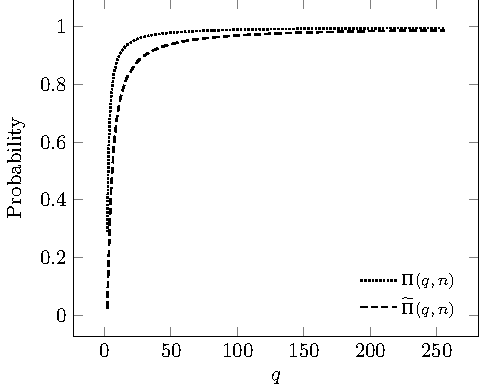
\includegraphics[width=.49\columnwidth]{charts/inv-prob/inv-prob}
  }
  \subfloat[
    Figure~\ref{fig:prob-inv-normal-size}, with $q \geq 16$.\label{fig:prob-inv-zoomed}
  ]{
    % 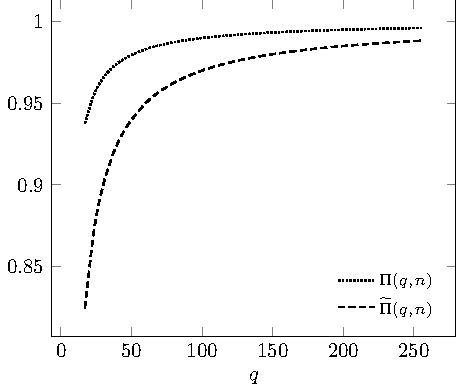
\includegraphics[width=.458\columnwidth]{charts/inv-prob/inv-prob-zoom}
  }
  \caption{Probability of obtaining $M \in \mathsf{GL}_{n}(\mathbb{F}_{q})$
    with $2 \leq q \leq 256$ and $q$ a prime power, given the
    quantity of layers of Rainbow.}\label{fig:prob-inv}
\end{figure}

It is also useful to calculate $\Pi(q) = \lim_{n \to \infty} \Pi(q, n)$ to observe changes in the probability with the growth of the number of equations. We note that this limit has a well-known series representation.

\begin{theorem}[{\cite[Theorem 14.3]{Apostol:2010}}]
  Euler's pentagonal number theorem states that
  \begin{align}
    \prod_{k = 1}^{\infty} 1 - q^{k} = \sum_{k = -\infty}^{\infty}
    {(-1)}^{k} q^{\frac{3k^{2} + k}{2}}.
  \end{align}
\end{theorem}

By simply swapping signs in the exponents, we can use this identity and obtain a fast approximation of the probability when $n$ tends to infinity. We use the SageMath language, which offers arbitrary precision real numbers, to obtain these values and find out that, when $n \geq 56$, $\Pi(q) \approx_{10^{-18}} \Pi(q, n)$ and $\widetilde{\Pi}(q) \approx_{10^{-8}} \widetilde{\Pi}(q, n)$. Thus, Figure~\ref{fig:prob-inv} also accurately reflects the behaviour of $\Pi(q)$, that is, current values of $n$ already reach effective upper bounds for this probability.

Hence, we note that the inversion event happens almost surely. Moreover, this evidence shows that computing a preimage in order to sign a message happens at the first try with high probability in a wide range of Rainbow configurations. Therefore, the cost of a central map reconfiguration, in the case that chosen vinegar variables do not lead to an invertible central map, is amortized by the overwhelming probability that a signature is successfully generated.

\subsection{Similarity of multiple signatures}\label{subsec:similar}

Vinegar variables chosen to compute a preimage of the central map are an integral part of the
preimage $\mathcal{C}(\mathbf{x}) = \mathbf{y}$. For instance, in the case $u = 2$, these make roughly a third of the output, considering common parameters for Rainbow. Further, we recall that there are approximately $q^{m}$ possibilities for $\mathbf{x}$, for any $\mathbb{F}_{q}$. Our proposal eliminates this choice by locking vinegar variables into the private key. Hence, it is essential to know if such variables create patterns in which private information may leak through a multi-target attack. Throughout this subsection, we use the SageMath PRNG, which implements a front-end to the \texttt{/dev/urandom} Linux kernel space generator.

We recall that a message digest $\mathbf{h}$ is signed instead of the entire document. Evidently, a secure cryptographic hash function shall produce an output that appears to be random. The application $\mathbf{y} = \mathcal{L}_{1}^{-1}(\mathbf{h})$ does not affect this behaviour, since the map is also random. Hence, we need not simulate this calculation in our analysis. According to Subsection~\ref{subsec:invert}, the operation $\mathcal{C}(\mathbf{x}) = \mathbf{y}$ creates a valid preimage with overwhelming probability, where the first $v_{1}$ elements of any $\mathbf{x}$ are the same.

We observe the distribution of field elements in vectors after the final function application, that is, $\mathbf{z} = \mathcal{L}_{2}^{-1}(\mathbf{x})$. Consider a $t$-tuple of signatures from an unmodified instance of Rainbow acting as a control group, that is, $Z_{t}' = (\mathbf{z}_{1}, \dots, \mathbf{z}_{t}),\; t \in \mathbb{N}$. Let its ``unpacked notation'' be the $(n \times t)$-tuple $Z_{t} = (z_{1}^{1}, z_{1}^{2}, \dots, z_{1}^{n}, z_{2}^{1}, \dots, z_{t}^{n - 1}, z_{t}^{n})$ of elements of $\mathbb{F}_{q}$. When the first $v_{1}$ elements of the vector $\mathbf{x}$ are fixed due to the usage of Rainbow-$\eta$, we instead denote these by $\widetilde{Z}'_{t}$ and $\widetilde{Z}_{t}$. 

Our hypothesis is that $Z_{t}$ and $\widetilde{Z}_{t}$ behave similarly to observations sampled from a discrete uniform distribution. This is due to the random process used in choosing the parts of a private key. Indeed, any element of $\mathbb{F}_{q}$ is equally likely to be picked to compose the matrix representation of a linear transformation, or be the coefficient of a monomial in an Oil--Vinegar polynomial.

\begin{definition}
  Let $\mathcal{U}(a, b)$ be a discrete uniform distribution with $a, b \in \mathbb{Z},\; a \leq b$. The \emph{standard deviation of $\mathcal{U}(a, b)$} is
  \begin{align}
    \sigma = \sqrt{\frac{(b - a + 1)^{2} - 1}{12}}.
  \end{align}
\end{definition}

Let $\mathcal{U}(1, q)$ be the discrete uniform distribution that represents the chance of randomly picking any element from $\mathbb{F}_{q}$. We note that if the field characteristic is even, there exists a mapping to the natural numbers that allows this choice to be performed. Thus, we expect that
\begin{align}
  \lim_{t \to \infty} \sigma(\widetilde{Z}_{t}) = \sqrt{\frac{q^{2} - 1}{12}},
\end{align}
suggesting that greater values of $n$ and $t$ approximate faster to the theoretical standard deviation.

\begin{figure}[ht]
  \subfloat[
    $d_{\sigma}(t)$ for $n = 42, v_{1} = 17$.\label{fig:std-diff-n42}
  ]{
    % 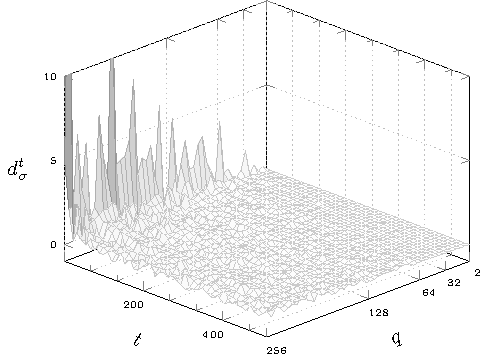
\includegraphics[width=.49\columnwidth]{charts/measure-diff/std-diff-n42}
  }
  \subfloat[
    $d_{\sigma}(t)$ for $n = 90, v_{1} = 35$.\label{fig:std-diff-n90}
  ]{
    % 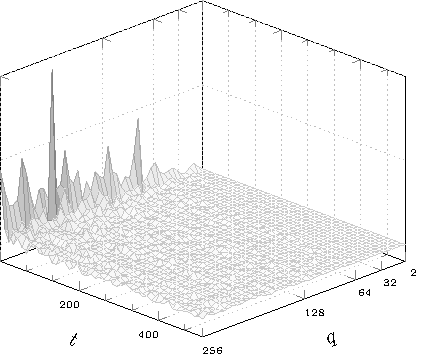
\includegraphics[width=.425\columnwidth]{charts/measure-diff/std-diff-n90}
  }
  \caption{Difference of standard deviations when $1 \leq t \leq 512$,
    and $2 \leq q \leq 256$ with $q$ as a prime power.}\label{fig:std-diff}
\end{figure}

Let us denote the absolute difference between standard deviations for $t$ as $d_{\sigma}(t) = \abs{\sigma(Z_{t}) - \sigma(\widetilde{Z}_{t})}$. Figure~\ref{fig:std-diff} shows the amplitude of such values for various values of $q$ and $t$. We note that the largest values of $d_{\sigma}(t)$ occur for finite fields of higher orders and lower $t$. For instance, given the vector space $\mathbb{F}_{223}^{42}$, we have $d_{\sigma}(1) \approx 8.25$, and for a slightly higher $t$, we obtain a much lower value $d_{\sigma}(11) \approx 0.24$. This behaviour is also observed within absolute differences of means, defined analogously as $d_{\mu}(t)$. The vector space $\mathbb{F}_{191}^{42}$ gives the values $d_{\mu}(1) \approx 5.31$ and, comparatively, $d_{\mu}(1) \approx 1.14$.

The comparison of expected with obtained standard deviations and means in our experiments gives positive results and confirms the law of large numbers. Still, it is interesting to look at the diffusion of values within $\widetilde{Z}_{t}$ and infer that it does not simply simulate the mean and standard deviation for a known discrete uniform. We count the amount of values for each class $1 \leq k \leq q$ and refer to them by $Z_{t, k}$ and $\widetilde{Z}_{t, k}$. By the central limit theorem, these counts should be normally distributed.

Figure~\ref{fig:dist-plot} shows the cumulative distribution function (CDF) plot and the Q-Q (quantile-quantile) plot for such samples. The expected CDF, as well as examples for $Z_{t}$ and $\widetilde{Z}_{t}$, show that all values are fairly distributed, with small variations due to the random generation of field elements. However, we note that this is due to the low number of classes, that is, the order of the finite field, and experimentally confirm that such discrepancies are largely reduced with $q = 2^{10}$.  

This is further confirmed by the Q-Q plot, which in this case is more commonly referred to as a normal probability plot. It is built by pairing the normalized counts $Z_{t, k}$ with quantiles from the standard normal distribution. Such quantiles are the normal order statistics, or rankits~\cite[p.~349]{Ipsen:194405}, which are hereafter referred to as $K \in \mathbb{R}^{q}$. Generating precise values for $K$ is non-trivial, and thus a method to yield approximate values is used.

\begin{figure}[htbp]
  \subfloat[
    CDF plot.\label{fig:cdf-plot}
  ]{
    % 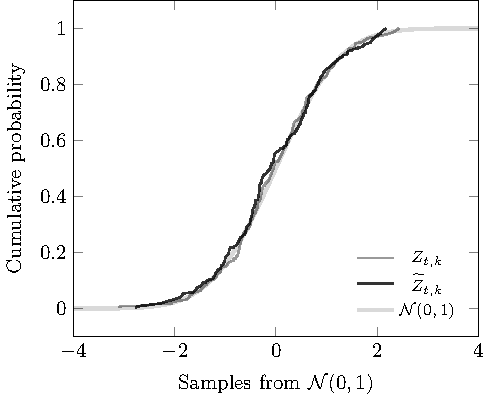
\includegraphics[width=.49\columnwidth]{charts/diffusion/cdf-plot}
  }
  \subfloat[
    Q-Q plot.\label{fig:qq-plot}
  ]{
    % 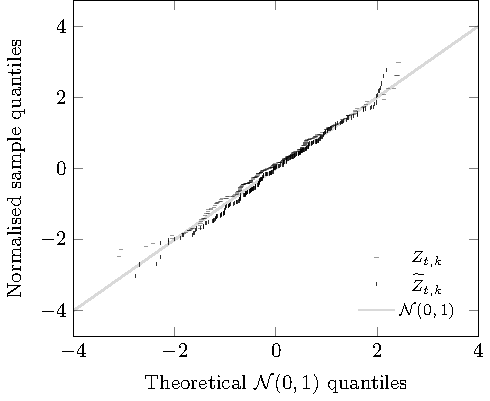
\includegraphics[width=.47\columnwidth]{charts/diffusion/qq-plot}
  }
  \caption{Distribution of counts of elements in $Z_{t}$ and
    $\widetilde{Z}_{t}$ such that $t = 2^{16}$ for
    $\mathbb{F}_{256}^{90}$.}\label{fig:dist-plot}
\end{figure}

Let $r \in \mathbb{N}$ be a precision parameter, and $\min(S, i)$ represent the $i$-th smallest value in a non-empty set $S$ with a partial order. A number $r \times q$ of samples are taken from a standard normal distribution $\mathcal{N}(0, 1)$ and organized into $q$-tuples $K_{1}, \dots, K_{r}$. Then, $K$ is composed of the means of the $i$-th smallest values in all $K_{j}$, that is,
\begin{align}
  K = \left( \mu(\{\min(K_{j}, i) : 1 \leq j \leq r\}) : 1 \leq i \leq q \right).
\end{align}
We have found experimentally that the lowest precision parameter $r = 1$ is still useful to interpret the graph. The resulting plot shows that points are sufficiently close to the $y = x$ expected line.

Our argument indicates that, even if part of the preimage created by the central map is fixed, the remaining linear transformation disrupts this pattern with high efficacy. Hence, an attacker with possession of multiple signatures created by our method would not be more capable of forging a new signature or deducing private information through statistical methods, than an attacker with no such knowledge.

\section{Enhancement of existing schemes}\label{sec:exp}

Our method does not depend on special structures inserted on the private key. Consequently, it can be applied to all known Rainbow-like schemes. We experiment with several sets of parameters and observe the reduction of private key sizes. It is known that there are various limitations for the choice of parameters that lead to secure instances of Rainbow~\cite{Petzoldt:201005}. We implement several known guidelines and confirm that our proposal does indeed work for a large range of parameters. Furthermore, we remark that comparisons are made considering the usage of homogeneous quadratic polynomials, and simplified linear transformations due to Theorem~\ref{thm:eq-keys-rainbow}.

\begin{table}[htbp]
  \renewcommand{\arraystretch}{1.2}
  \setlength{\tabcolsep}{6.5pt}
  \centering
  \caption{Reduction of Rainbow key sizes, in bytes, for various instances of the scheme.}\label{tab:eta-diff}
  \begin{tabular}{*{2}{l}*{5}{r}}
    \toprule
    Instance & Parameters & $n$ & $m$ & $\#\mathsf{sk}$ & $\#\mathsf{sk}^{\eta}$ & Difference \\ \midrule
    I-a   & $(\mathbb{F}_{ 16}, 32, 32, 32)$ &  96 &  64 & \num{   92928} & \num{  26896} & $-71.06\%$ \\
    I-b   & $(\mathbb{F}_{ 31}, 36, 28, 28)$ &  92 &  56 & \num{  105916} & \num{  24628} & $-76.75\%$ \\
    I-c   & $(\mathbb{F}_{256}, 40, 24, 24)$ &  88 &  48 & \num{  132576} & \num{  24136} & $-81.79\%$ \\
    III-b & $(\mathbb{F}_{ 31}, 64, 32, 48)$ & 144 &  80 & \num{  389975} & \num{  71552} & $-81.65\%$ \\
    III-c & $(\mathbb{F}_{256}, 68, 36, 36)$ & 140 &  72 & \num{  511416} & \num{  78188} & $-84.71\%$ \\
    IV-a  & $(\mathbb{F}_{ 16}, 56, 48, 48)$ & 152 &  96 & \num{  358656} & \num{  88540} & $-75.31\%$ \\
    V-c   & $(\mathbb{F}_{256}, 92, 48, 48)$ & 188 &  96 & \num{ 1227072} & \num{ 180572} & $-85.28\%$ \\
    VI-a  & $(\mathbb{F}_{ 16}, 76, 64, 64)$ & 204 & 128 & \num{  860800} & \num{ 206630} & $-76.00\%$ \\
    VI-b  & $(\mathbb{F}_{ 31}, 84, 56, 56)$ & 196 & 112 & \num{  980524} & \num{ 187172} & $-80.91\%$ \\
    P-080 & $(\mathbb{F}_{256}, 17, 13, 13)$ &  43 &  26 & \num{   16757} & \num{   4177} & $-75.07\%$ \\
    P-100 & $(\mathbb{F}_{256}, 26, 16, 17)$ &  59 &  33 & \num{   41163} & \num{   8364} & $-79.68\%$ \\
    P-128 & $(\mathbb{F}_{256}, 36, 21, 22)$ &  79 &  43 & \num{   96288} & \num{  17754} & $-81.56\%$ \\
    P-192 & $(\mathbb{F}_{256}, 63, 46, 22)$ & 131 &  68 & \num{  416998} & \num{  52417} & $-87.43\%$ \\
    P-256 & $(\mathbb{F}_{256}, 85, 63, 30)$ & 178 &  93 & \num{ 1043295} & \num{ 128950} & $-87.64\%$ \\
    I     & $(\mathbb{F}_{ 16}, 36, 32, 32)$ & 100 &  64 & \num{  103616} & \num{  27026} & $-73.92\%$ \\
    III   & $(\mathbb{F}_{256}, 68, 32, 48)$ & 148 &  80 & \num{  626016} & \num{ 107652} & $-82.80\%$ \\
    V     & $(\mathbb{F}_{256}, 96, 36, 64)$ & 196 & 100 & \num{ 1408704} & \num{ 204384} & $-85.49\%$ \\
    \bottomrule
  \end{tabular}
\end{table}

We show results for the application of our method in Table~\ref{tab:eta-diff}, considering parameter sets of Tables~\ref{tab:sec} and~\ref{tab:newsec}. Indeed, the choice of $v_{1}$ remarkably affects the results. Moreover, a minimal value of $o_{u}$ is also known to further reduce the private key size. Indeed, we suggest that $v_{1} \geq o_{u}$ as much as possible to maximize the results of our method. However, we remark that one must set sufficient parameters for $o_{i}$ such that the scheme still resists direct and UOV attacks.

The case of Rainbow variants is slightly more convoluted. Schemes claim optimizations of the private key often through the inclusion of inner structuring. To measure the impact of our method within the context of these schemes, it is imperative to understand such structures. For instance, it may be the case that a method introduces sparseness related to specific vinegar variables. Thus, the reduction would not be equally distributed over the private key elements and, as such, our method would have its efficiency reduced.

To the best of our knowledge, it is not trivial to combine our strategy with the schemes presented in Subsection~\ref{subsec:priv}, and resulting gains would be evidently reduced. Furthermore, several of those schemes were subsequently broken or new parameters were proposed, suggesting that such a combination would not be productive. We thus consider only schemes that reduce the public key size, that is, CyclicRainbow~\cite{Petzoldt:201012} and RainbowLRS2~\cite[Section 9.2]{Petzoldt:201307}.

\begin{table}[htbp]
  \renewcommand{\arraystretch}{1.2}
  \centering
  \caption{Total reduction of Rainbow key pairs, in bytes, for variants of the scheme.}\label{tab:pair-diff}
  \begin{tabular}{*{2}{l}*{4}{r}}
    \toprule
    Instance & Variant & $\#\mathsf{sk}$ & $\#\mathsf{sk}^{\eta}$ & $\#\mathsf{pk}$ & Difference \\ \midrule
    \multirow{3}{*}{P-080} & Classic & \multirow{3}{*}{\num{  16757}} & \multirow{3}{*}{\num{   4177}} & \num{   24596} & $-30.42\%$ \\
                           & Cyclic  &                                &                                & \num{    9474} & $-66.99\%$ \\
                           & LRS2    &                                &                                & \num{    8645} & $-68.99\%$ \\
    \multirow{3}{*}{P-100} & Classic & \multirow{3}{*}{\num{  41163}} & \multirow{3}{*}{\num{   8364}} & \num{   58410} & $-32.94\%$ \\
                           & Cyclic  &                                &                                & \num{   20266} & $-71.25\%$ \\
                           & LRS2    &                                &                                & \num{   18682} & $-72.84\%$ \\
    \multirow{3}{*}{P-128} & Classic & \multirow{3}{*}{\num{  96288}} & \multirow{3}{*}{\num{  17754}} & \num{  135880} & $-33.83\%$ \\
                           & Cyclic  &                                &                                & \num{   44971} & $-72.98\%$ \\
                           & LRS2    &                                &                                & \num{   42107} & $-74.22\%$ \\
    \multirow{2}{*}{I    } & Classic & \multirow{2}{*}{\num{ 103616}} & \multirow{2}{*}{\num{  27026}} & \num{  161600} & $-28.88\%$ \\
                           & nCyclic &                                &                                & \num{   60160} & $-67.13\%$ \\
    \multirow{2}{*}{III  } & Classic & \multirow{2}{*}{\num{ 626016}} & \multirow{2}{*}{\num{ 107652}} & \num{  882080} & $-34.37\%$ \\
                           & nCyclic &                                &                                & \num{  264576} & $-75.32\%$ \\
    \multirow{2}{*}{V    } & Classic & \multirow{2}{*}{\num{1408704}} & \multirow{2}{*}{\num{ 204384}} & \num{ 1930600} & $-36.07\%$ \\
                           & nCyclic &                                &                                & \num{  536104} & $-77.83\%$ \\
    \bottomrule
  \end{tabular}
\end{table}

We compare key pair sizes when our method is used alongside Rainbow variants that reduce the public key size. Table~\ref{tab:pair-diff} presents results for some sets of parameters from Table~\ref{tab:eta-diff}. We calculate $\#\mathsf{pk}$ for the variants according to~\cite[Eqs.~9.2,~9.4]{Petzoldt:201307} and~\cite{Petzoldt:202004}. As per~\cite[Remark 9.1]{Petzoldt:201307}, we note that $q = 16$ and $q = 31$ are not considered due to a security restriction of RainbowLRS2. The ``nCyclic'' method is a small improvement over CyclicRainbow featured on the second round submission of Rainbow to the NIST standardization process~\cite{Ding:201901}. We obtain positive results, with key pair size reductions of up to a factor of 3.

The use of CyclicRainbow or RainbowLRS2 with Rainbow-$\eta_{2}$ is recommended. These variants are based on the linear relations described in Subsection~\ref{sec:mod}, and resulting implementations may be effortlessly modified to use our proposal. Moreover, in the case that higher parameters are needed, for example a security level of $256$ bits, we note that the key pair is reduced more aggressively. Thus, our results reflect changes over a wide variety of platforms and possible Rainbow deployments that benefit from lower storage requirements.

We also briefly discuss the effect of these changes on the signature generation step overall performance. In the case of Rainbow-$\eta_{1}$, it does not vary greatly due to the fast regeneration of the central map elements from a given PRNG and $\mathbf{S}$. On the other hand, Rainbow-$\eta_{2}$ uses elaborate techniques to reconstruct the central map if vinegar variables are not suitable. This process is not without cost, and it may negatively affect the average signature generation time, for instance as seen in~\cite{Petzoldt:202004}. Still, by making use of Rainbow-$\eta_{3}$, these computations are entirely avoided by choosing a new salt instead of new vinegar variables, reducing the inherent overhead.

\chapter{Variant of Kipnis--Shamir attack}\label{ch:attack}
% TODO expand

As seen in Chapter~\ref{ch:eta}, several arguments were made in order to present support to the security of our Rainbow-$\eta$ proposal. We recall that the inner workings of the scheme are not modified, and a sideline modification is done instead, which preserves randomness of signatures. This is based on the fact that, as summarized in Section~\ref{sec:related}, there is encouraging evidence that adding further structure to the central map is dangerous to the security of Oil--Vinegar schemes. 

We intentionally avoid this strategy with our proposal. Nonetheless, we present partial evidence that our proposal is not secure due to leakage of information from the private key through signatures. In Section~\ref{sec:atdesc}, we briefly describe the Kipnis--Shamir attack and present a variation of this attack that produces an equivalent key for a scheme that makes use of our proposal. In Section~\ref{sec:counter}, we show the practical consequences of this attack and possible countermeasures that still allow for a trade-off between security and private key size.

\section{Attack description}\label{sec:atdesc}

In this section, we show how to mount a key recovery attack against a scheme that makes use of the Rainbow-$\eta$ strategy. In Subsection~\ref{subsec:ks}, we recall the Kipnis--Shamir attack, the first cryptanalytic method that specifically targeted Oil--Vinegar signature schemes. In Subsection~\ref{subsec:etaks}, we present our version of the attack that works against the proposal of Chapter~\ref{ch:eta}.

\subsection{Original method}\label{subsec:ks}

The Kipnis--Shamir attack, or UOV attack, was first given in~\cite{Kipnis:199808} as a proof of insecurity of the balanced Oil--Vinegar signature scheme. The fact that $v = o$ allows for the leakage of information in the public key that can be used to reconstruct an equivalent private key. This method led to the creation of UOV as a countermeasure~\cite{Kipnis:199904} with $v = 2o$. The attack was generalized on the same work, but it is computationally hard to perform if the difference $v - o$ is not small enough. The UOV attack stands relevant in the cryptanalysis of Oil--Vinegar signature schemes, as seen in Section~\ref{sec:related}. 

We give a description of the Kipnis--Shamir attack for finite fields of odd characteristic~\cite[Section 3.2]{Ding:2006} for readability, and refer the reader to~\cite{Cao:201105} for the case of even characteristic.

\subsection{Our attack}\label{subsec:etaks}

The modification of Rainbow-$\eta$ fixes vinegar variables in the signature generation step of the scheme. By pre-substituting these in the central map, it can be stored more efficiently. This is allowed, since the map can be reconstructed if signature generation fails, allowing the signing of any messages. We propose three methods to achieve this, through either a seed, mathematical relations between the public key and the central map, as explained in Subsection~\ref{sec:mod}, or simply by changing the message with a nonce due to the EU-CMA trait. The difference between signatures made with the same vinegar variables and usual signatures is not statistically significant, as argued in Subsection~\ref{subsec:similar}. Moreover, there is no limitation on parameters such that their secure selection is always encouraged.



Our attack is inspired by the method of Kipnis--Shamir~\cite{Kipnis:199808}, which is a key recovery attack that separates oil and vinegar variables through manipulation of linear combinations of the public key. It is based on the fact that, in the case of the balanced Oil--Vinegar scheme, a mapping of the oil subspace $\mathcal{O} = \{ (x_{1}, \dots, x_{n}) \in \mathbb{F}^{n} : x_{1} = \cdots = x_{v} = 0 \}$ to itself can be found in polynomial time. This allows for the reconstruction of the accompanying linear transformation $\mathcal{L}_{2}$. It is discussed in more detail in Subsection~\ref{subsec:uov}.

It is classified as a key recovery attack, in the sense that an equivalent key is recovered, and allows for a malicious entity to create signature forgeries in polynomial time. In our variant, the attacker must collect a large enough set of signatures in order to recover an equivalent key. The key observation is that signatures produced with Rainbow-$\eta$ can be used directly in the construction of a basis for $\mathcal{L}_{2}^{-1}(\mathcal{O})$. Consequently, an equivalent linear transformation $\widetilde{\mathcal{L}}_{2}$ can be built and composed with the public key to yield an equivalent private key.

We briefly describe the attack for UOV, that is, a Rainbow scheme with a single layer and $\mathcal{L}_{1} = \textsf{id}$. We note that this linear transformation is irrelevant to UOV and the attack itself. Consider an UOV scheme with $v, o \in \mathbb{N}$ and $\mathsf{sk} = (\mathcal{C}, \mathcal{L}_{2}), \mathsf{pk} = \mathcal{C} \circ \mathcal{L}_{2}$ as per Section~\ref{sec:ov}. We recall that $n = v + o$ is the number of variables, and $m = o$ the number of equations in $\mathcal{C}$ and $\mathsf{pk}$. An attacker must collect at least $m + 1$ signatures known to be produced with the same vinegar variables through Rainbow-$\eta$ for the attack to work. Let this set be denoted as $\rho = (\sigma_{1}, \dots, \sigma_{m + 1})$. 

The first $v$ variables of any $\sigma_{i}$ under the transformation $\mathcal{L}_{2}^{-1}$ are equal to the chosen sequence of vinegar variables $V_{1} = (x_{1}, \dots, x_{v})$, i.e. the preimage $\mathcal{L}_{2}^{-1}(\sigma_{i}) = (x_{1}, \dots, x_{v}, \ast, \dots, \ast)$. Since this is the case for any $\sigma_{i}$, we have that $\mathcal{L}_{2}^{-1}(\sigma_{i} - \sigma_{i + 1}) = (0, \dots, 0, \ast, \dots, \ast)$. In fact, any subtraction between two signatures in $\rho$ yields vectors starting with $v$ zeroes. Let us call such a vector $\chi_{i}$, and evidently $\chi_{i} \in \mathcal{L}_{2}^{-1}(\mathcal{O})$. Since the attacker's goal is to build a basis of this set, then $m$ linearly independent $\chi_{i}$ must be collected such that the basis can be constructed. Let us call this set $\widetilde{\rho}$. We note that at least $m + 1$ signatures need to be collected to perform $m$ subtractions.

The construction of the basis $B$ for $\mathcal{L}_{2}^{-1}(\mathcal{O})$ is given below. We operate on the matrix representation of $B$, denoted $M(B)$. A standard basis is taken as a blueprint, its last $m$ rows are substituted with the vectors in $\widetilde{\rho}$, and the matrix is then transposed. More concisely, a simple basis extension is performed. Equivalently,
\begin{align}
  B^{\mathsf{T}} = \begin{bmatrix}
    1 & 0 & 0 & \cdots & 0 \\
    0 & 1 & 0 & \cdots & 0 \\
    0 & 0 & 1 & \cdots & 0 \\
    \vdots & \vdots & \vdots & \ddots & \vdots \\
    \chi_{11} & \chi_{12} & \chi_{13} & \cdots & \chi_{1n} \\
        \vdots & \vdots & \vdots & \ddots & \vdots \\
    \chi_{m1} & \chi_{m2} & \chi_{m3} & \cdots & \chi_{mn} \\
  \end{bmatrix}.
\end{align}
Then, if $B \in \mathsf{GL}(\mathbb{F}^{n})$, the inverse of $\widetilde{\mathcal{L}}_{2}$ can be constructed. If this is not the case, then other vectors in $\rho$ need to be picked to form $\widetilde{\rho}$. This is due to the fact that the desired equivalent private key is of the form $\mathbf{sk'} = (\mathsf{pk} \circ \widetilde{\mathcal{L}}_{2}, \widetilde{\mathcal{L}}_{2}^{-1})$. By representing $B$ as a linear transformation and performing the aforementioned composition, we obtain an equivalent key. Evidently, $\mathsf{pk} \circ \widetilde{\mathcal{L}}_{2}$ must be a system of Oil--Vinegar polynomials~\cite[Theorem 1]{Beullens:201706}. Finally, an attacker can use $\mathbf{sk'}$ and produce signature forgeries of any desired message, not necessarily needing to fix any vinegar variables and thus producing ``secure forgeries''.

\section{Aftermath and countermeasures}\label{sec:counter}

In this section, we show the efforts associated with performing our attack, and possible strategies to repair our proposal, such that there is a clear trade-off between private key sizes and security levels. In Subsection~\ref{subsec:mount}, we discuss the probabilities of applying the attack to vulnerable Rainbow-like schemes in practical settings. In Subsection~\ref{subsec:repair}, we examine the effects of fixing a fraction of all vinegar variables in order to preserve negligible attack probabilities.

\subsection{Mounting the attack in practice}\label{subsec:mount}

As discussed in Section~\ref{subsec:etaks}, the collection of signatures produced with Rainbow-$\eta$ is pivotal to carry on with the attack. Thus, we show the probabilities associated with picking a valid subset of items from a large number of amassed signatures to, in turn, obtain an equivalent key. We remark that there is no way to identify if a signature is produced with Rainbow-$\eta$ except by observation of the public implementations. However, it is simple enough to modify the key and signature generation algorithms to yield either conventional or reduced private keys by choice of the signer. 

If an attacker has no access to the signing device, it is not possible to discern whether our optimization is used or not. Otherwise, several other side-channel attacks may be carried out, possibly foiling Rainbow implementations even if our method is never applied. Let us then consider that a signer produces a number $N \in \mathbb{N}$ of signatures such that $K \leq N$ of those are created with the same vinegar variables. Without loss of generality, let $K = \ceil{\alpha N}$ with $0 \leq \alpha \leq 1$.

By precisely choosing a target, an attacker may increase the odds of obtaining useful signatures for the attack. Nonetheless, we observe such probabilities for various values of $\alpha$, and model this behaviour as follows. Given the aforementioned $N$ and $K$, we wish to obtain $k \leq K$ signatures that were produced with Rainbow-$\eta$ from a sample size $n \leq N$. By the description of our attack in Subsection~\ref{subsec:etaks}, the attacker needs $k$ distinct signatures, or in other words, sampling is \emph{without replacement}. The probability distribution that describes this situation is given below.

\begin{definition}
  Given $N, K, n, k \in \mathbb{N}$ with $K, n \leq N$ and $0 \leq k \leq K$, if the probability mass function (PMF) of a discrete random variable $\mathbf{X}$ is
  \begin{align}
    \Pr[\mathbf{X} = k] = \frac{\binom{K}{k}\binom{N - K}{n - k}}{\binom{N}{n}},
  \end{align}
  then $\mathbf{X}$ follows the \emph{hypergeometric distribution}. The peak of this PMF, or its \emph{mode}, is
  \begin{align}
    \hat{\mathbf{X}} = \left\lfloor \frac{(n + 1)(K + 1)}{N + 2} \right\rfloor.
  \end{align}
\end{definition}

The probability of sampling a valid subset of signatures is then equivalent to calculating $\Pr[\mathbf{X} > k]$, which is the description of the complementary CDF. We remark that for large populations, the evaluation of the naive formula $\sum_{i = k + 1}^{K} \Pr[\mathbf{X} = i]$ may be computationally expensive and prone to overflow. Thus, an algorithm such as~\cite{Berkopec:200607} should be used in these cases.

\begin{figure}[htbp]
  \subfloat[
    PMF plot.\label{fig:hyper-pmf-plot}
  ]{
    % 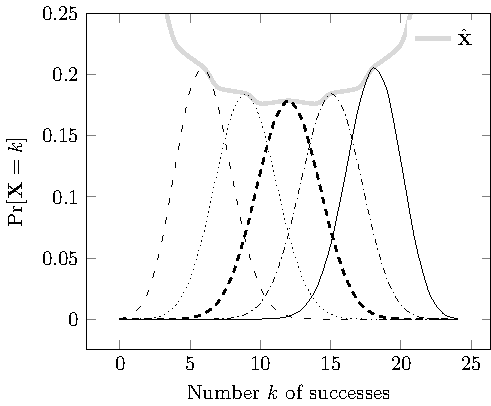
\includegraphics[width=.48\columnwidth]{charts/hyper/hyper-pmf}
  }
  \subfloat[
    CDF plot.\label{fig:hyper-cdf-plot}
  ]{
    % 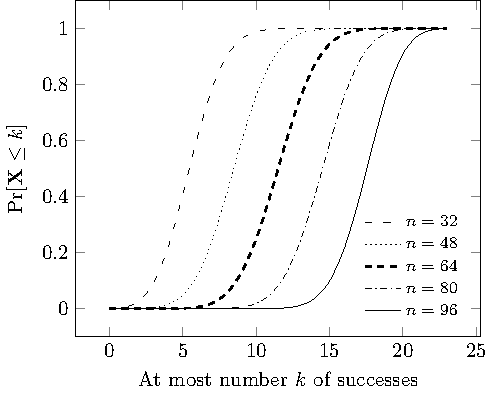
\includegraphics[width=.48\columnwidth]{charts/hyper/hyper-cdf}
  }
  \caption{Hypergeometric distribution with
    $N = 128$, $K = 24$ and $n \in \{32, 48, 64, 80, 96\}$.}\label{fig:hyper}
\end{figure}

We now explore the probability that, given $n$ draws from a population of size $N$ with $K$ signatures produced with Rainbow-$\eta$, there exist at least $k$ successes. Figure~\ref{fig:hyper} shows the PMF to the left, and the CDF to the right, of a sample hypergeometric distribution. For instance, we note that for a factor $\alpha = 0.2$, if an attacker performs sampling without replacement of $\frac{1}{4}$ of the population, that is $n = 32$, there exists a chance of $\approx 1\%$ that $k = 10$ or more signatures with the desired feature are obtained. On the other hand, if $\frac{1}{2}$ of the population is sampled, or $n = 64$, the probability is $\approx 75\%$. Indeed, the probability of obtaining a higher number of successes grows with the number of draws, as expected.

However, the sample size is easily controlled by the attacker. It is more advantageous to reason about the $\alpha$ factor, which may be unknown. To this end, a remarkable fact about the hypergeometric distribution is that it is \emph{symmetric} on the $K$ and $n$ parameters. This may be verified by expanding the PMF definition into binomials for both cases and checking for the desired equality. Thus, Figure~\ref{fig:hyper} also represents the behaviour of various $\alpha$ factors in the form of different quantities of signatures eligible for the attack, that is, $K \in \{32, 48, \dots, 96\}$ and a fixed number of samples $n = 24$.

It is thus expected that a large enough number of signatures is collected for a reasonable chance of obtaining a valid sample. For example, given $N = 2^{12}$ and $K = 2^{10}$, or $\alpha = 0.25$, and $n = 2^{8}$, then $\hat{\mathbf{X}} = 64$, which is equal to the number of equations $m$ of a Rainbow instance with minimal security level, according to Table~\ref{tab:newsec}. The attack description in Subsection~\ref{subsec:etaks} requires $m + 1$ ``weak'' signatures as a parameter. Thus, the associated probability of obtaining at least $65$ successes is $\Pr[\mathbf{X} > 64] \approx 46.6\%$.

The identification problem remains difficult if $n$ is much larger than $k$, since the attacker still does not know which signatures are useful to perform the attack. Ideally, a sample should return exactly the desired number of ``weak'' signatures, that is, $n = k$. In this case, the PMF is given by
\begin{align}
  \frac{\binom{K}{k}}{\binom{N}{k}} = \frac{K! (N - k)!}{N! (K - k)!},
\end{align}
which yields negligible probabilities even for relatively small parameters. For example, given $N = 2^{8}$ and $K = 2^{7}$, or $\alpha = 0.5$, and $n = k = 2^{6}$, $\Pr[\mathbf{X} = k] \approx 1.2576 \times 10^{-24}$.

If the attacker collects signatures from multiple signers but cannot classify the signatures according to each public key, the problem can still be modelled through a \emph{multivariate hypergeometric distribution}. Finally, the success of an attacker is directly proportional to the maximization of the number of draws or the $\alpha$ factor, such that only probabilities pertaining to the attack itself need consideration. The \texttt{CertificateVerify} message of a TLS handshake~\cite[Subsection~4.4.3]{Rescorla:201808} may be leveraged in order to implement a practical proof-of-concept for the attack, which is outside the scope of this work.

\subsection{Reparation of the method}\label{subsec:repair}

It is clear from Subsection~\ref{subsec:mount} that some effort is needed to perform the attack of Subsection~\ref{subsec:etaks} in practice. However, the existence of such a mathematical method presents a concrete advantage for an attacker to obtain an equivalent key from a well-targeted entity. We attempt to subside this behaviour by extending our original proposal with a configuration parameter which controls how vinegar variables are fixed. In the following, we introduce this modification and discuss the probabilities associated with performing our attack, if some level of randomness is maintained in the central map preimage. Therefore, the private key size still benefits from several fixed elements and security is not thwarted.

We recall that $\widetilde{V}_{1}$ is the sequence of vinegar variables used on the signature generation algorithm of Rainbow-$\eta$. In the original scheme, it is chosen randomly for every signing process and thus it is not part of the private key, yielding roughly $q^{v_{1}}$ possible preimages for a message digest. In the case of Rainbow-$\eta$, there is only one preimage if the partial evaluation of the central map gives an exactly determined polynomial system. We recall a well-known concept that allows for the quantification of such preimages, and other features of our new proposal.

\begin{definition}
  Given $k \in \mathbb{N}$ and a binary vector $\mathbf{x} \in \mathbb{F}_{2}^{k}$, the number of non-zero elements of $\mathbf{x}$, or
  \begin{align}
    \text{wt}(\mathbf{x}) = |\{ i \mid x_{i} \neq 0, 1 \leq i \leq k \}|,
  \end{align}
  is the \emph{Hamming weight of $\mathbf{x}$}.
\end{definition}

Let $\mathbf{v} \in \mathbb{F}_{2}^{v_{1}}$ be the \emph{vinegar threshold}, a sequence of bits that encodes which elements from $\widetilde{V}_{1}$ are to be fixed. More precisely, for $1 \leq i \leq v_{1}$, if $\mathbf{v}_{i} = 0$ then the i-th element of $\widetilde{V}_{1}$ is swapped with a randomly chosen element from $\mathbb{F}_{q}$, and if $\mathbf{v}_{i} = 1$, it remains unchanged. Evidently, if $\mathbf{v} = (0, \dots, 0)$, we turn back to the original Rainbow scheme, and for $\mathbf{v} = (1, \dots, 1)$, we get the schemes of Section~\ref{sec:mod}. Therefore, the number of possible signatures for a given message digest is $\approx q^{v_{1} - \text{wt}(\mathbf{v})}$. Let us denote this method as Rainbow-$\eta_{4}$. We remark that it is compatible with any of the schemes of Section~\ref{sec:mod}.

\subsubsection{Key generation.}

Generate a $\mathbf{v} \random{} \mathbb{F}_{2}^{v_{1}}$ such that $\text{wt}(\mathbf{v}) \neq v_{1}$. Generate the maps $(\mathcal{L}_{1}, \mathcal{C}, \mathcal{L}_{2})$ and $\mathcal{P}$ through the usual key generation algorithm. Generate the sequence $\widetilde{V}_{1}$ according to the limitations encoded in $\mathbf{v}$, and substitute terms into $\mathcal{C}$, giving $\overline{\mathcal{C}}$. Then,
\begin{align}
  \begin{split}
    \mathsf{sk}^{\eta_{4}} &= (\widetilde{V}_{1}, \mathcal{L}_{1}, \overline{\mathcal{C}}, \mathcal{L}_{2}, \mathbf{v}), \\
    \mathsf{pk}^{\eta_{4}} &= \mathcal{P}.
  \end{split}
\end{align}

\subsubsection{Signature generation.}

This step does not change significantly from Rainbow-$\eta$. Consider a message $M$ and obtain its digest $\mathbf{h} = \mathcal{H}(M)$. Compute $\mathbf{y} = \mathcal{L}_{1}^{-1}(\mathbf{h})$, and randomly choose the vinegar variables as encoded in $\mathbf{v}$. Attempt to generate the preimage $\overline{\mathcal{C}}(\mathbf{x}) = \mathbf{y}$ by inverting every layer recursively. If this is not possible, vinegar variables have to be chosen again by the aforementioned procedure. Finally, compute $\mathbf{z} = \mathcal{L}_{2}^{-1}(\mathbf{x})$.

\subsubsection{Signature verification.}

This step does not change. If $\mathbf{h} = \mathcal{P}(\mathbf{z})$, then the signature is valid, and otherwise invalid.

We note that there is no need to provide a reconstruction procedure of $\overline{\mathcal{C}}$ as in the case of Rainbow-$\eta_{1}$, which needs a seed, and Rainbow-$\eta_{2}$, that features non-trivial mathematical relations. The private key size of Rainbow-$\eta_{4}$ is similar to Proposition~\ref{prop:eta-key-size}, with a small increase due to storage of $\mathbf{v}$, but also reduced due to the size of $\widetilde{V}_{1}$, which is now $v_{1} - \text{wt}(\mathbf{v})$. We now expand on the security of our new proposal.

The fact that $\mathbf{v} = (1, \dots, 1)$ leads to the attack of Subsection~\ref{subsec:etaks}. However, if there is no information on which, and how many variables are fixed, the attacker is forced to guess such combinations, hampering its progress. Thus, it is useful to discuss the choice of $\mathbf{v}$ in the key generation algorithm. By simply leaving the choice as uniformly random, $v_{1}$ bits need to be chosen independently. The distribution which gives this behaviour is presented below.

\begin{definition}
  Given $n \in \mathbb{N}$ and $0 \leq p \leq 1$, if the PMF of a discrete random variable $\mathbf{X}$ is
  \begin{align}
    \Pr[\mathbf{X} = k] = \binom{n}{k} p^{k} (1 - p)^{n - k},
  \end{align}
  then $\mathbf{X}$ follows the \emph{binomial distribution}. It has mean $\mu = np$ and standard deviation $\sigma = \sqrt{np(1 - p)}$.
\end{definition}

To appropriately interpret sampling of $\mathbf{v}$, we set $n = v_{1}$ and $p = 0.5$. It is desirable that $\text{wt}(\mathbf{v})$ is not maximized, as seen in Table~\ref{tab:bin-prob}, which shows the probability of obtaining a signature with the same vinegar variables given several Hamming weights.

\begin{table}[htbp]
  \renewcommand{\arraystretch}{1.2}
  \setlength{\tabcolsep}{6.5pt}
  \centering
  \caption{Probability of obtaining a signature with a previously used $\mathbf{v}$.}\label{tab:bin-prob}
  \begin{tabular}{*{2}{l}*{5}{r}}
    \toprule
    \midrule
    \bottomrule
    \end{tabular}
\end{table}

% A simple experiment shows that $\text{wt}(\mathbf{v})$ will be within three standard deviations in more than $99\%$ of the cases, for $16 \leq v_{1} \leq 128$.


% TODO
\chapter{Conclusion}\label{ch:conc}

\subsubsection{Future work.}

\bibliographystyle{alpha}
{\scriptsize \bibliography{ref}}

\end{document}






